\documentclass[a4paper,11pt,portrait]{article}

%======================================================================
%   LLM INSTRUCTIONS & GROUNDING RULE
%======================================================================
% This template is to be used by the AI/LLM to generate exam solutions.
%
% *** GROUNDING RULE ***
% When generating a solution, if theory slides are provided, you MUST
% include a grounding truth based on the theory slides.
% Ensure that the solution is consistent with the provided materials.
%======================================================================

%======================================================================
%   MODE FLAGS (passed via command line)
%======================================================================
% \printmodeflag  -> Print mode (B&W)
% Neither         -> Read mode (default)
%======================================================================
\newif\ifprintmode

\ifdefined\printmodeflag
    \printmodetrue
\else
    \printmodefalse
\fi

%======================================================================
%   EXAM YEAR HEADER
%======================================================================
\newcommand{\examyear}[1]{\def\currentexamyear{#1}\markboth{#1}{#1}}
\def\currentexamyear{}

%======================================================================
%	PREAMBLE & PACKAGES
%======================================================================
\usepackage{fontspec}
\usepackage{polyglossia}
\setmainlanguage[numerals=arabic]{greek}
\setotherlanguage{english}

%======================================================================
%   FONT SELECTION (Read/Print Mode)
%======================================================================
\setmainfont[
    Path = Garidomakaronada_Template/fonts/atkinson-hyperlegible/fonts/ttf/,
    Extension = .ttf,
    UprightFont = *-Regular,
    BoldFont = *-Bold,
    ItalicFont = *-Italic,
    BoldItalicFont = *-BoldItalic
]{AtkinsonHyperlegible}
\setsansfont[
    Path = Garidomakaronada_Template/fonts/atkinson-hyperlegible/fonts/ttf/,
    Extension = .ttf,
    UprightFont = *-Regular,
    BoldFont = *-Bold,
    ItalicFont = *-Italic,
    BoldItalicFont = *-BoldItalic
]{AtkinsonHyperlegible}
\setmonofont{DejaVu Sans Mono}
\newfontfamily\greekfont[Scale=MatchLowercase]{DejaVu Serif}
\newfontfamily\greekfontsf[Scale=MatchLowercase]{DejaVu Sans}

\usepackage{amsmath}
\usepackage{unicode-math}
\usepackage{listings}
\usepackage{booktabs}
\usepackage{array}
\usepackage{xcolor}
\usepackage[most]{tcolorbox}
\usepackage[portrait, top=1.5cm, bottom=1.25cm, left=1cm, right=1cm, headheight=14pt]{geometry}
\usepackage{hyperref}
\usepackage{pdfpages}
\usepackage{fancyhdr}
\usepackage{graphicx}
\usepackage{tikz}
\usetikzlibrary{shapes,arrows,positioning,calc,backgrounds,patterns}
\usepackage{tcolorbox}
\tcbuselibrary{breakable,skins}
\usepackage{enumitem}
\usepackage{float}
\usepackage{pgfplots}
\pgfplotsset{compat=1.18}

%======================================================================
%   COLOR DEFINITIONS (Read/Print Mode)
%======================================================================
\ifprintmode
    \definecolor{answerbox}{gray}{1.0}
    \definecolor{questionbg}{gray}{1.0}
    \definecolor{partbg}{gray}{1.0}
    \definecolor{answerframe}{gray}{0.1}
    \definecolor{questionframe}{gray}{0.0}
    \definecolor{linkcolor}{gray}{0.0}
    \definecolor{headercolor}{gray}{0.1}
    \definecolor{codelistingbg}{gray}{1.0}
\else
    \definecolor{answerbox}{RGB}{230,245,230}
    \definecolor{questionbg}{RGB}{240,248,255}
    \definecolor{partbg}{RGB}{255,250,240}
    \definecolor{answerframe}{RGB}{60,130,60}
    \definecolor{questionframe}{RGB}{50,80,140}
    \definecolor{linkcolor}{RGB}{0,0,180}
    \definecolor{headercolor}{RGB}{80,80,80}
    \definecolor{codelistingbg}{RGB}{245,245,245}
\fi

\lstset{
    basicstyle=\ttfamily\small,
    breaklines=true,
    frame=single,
    backgroundcolor=\color{codelistingbg},
    numbers=none,
    showstringspaces=false
}

%======================================================================
%   TCOLORBOX DEFINITIONS (Read/Print Mode)
%======================================================================
\newtcolorbox{answer}{
    colback=answerbox,
    colframe=answerframe,
    title=Λύση,
    fonttitle=\bfseries,
    boxrule=0.8pt,
    breakable,
    arc=2pt,
    left=6pt,
    right=6pt,
    top=4pt,
    bottom=4pt
}

\newtcolorbox{question}[1][]{
    colback=questionbg,
    colframe=questionframe,
    fonttitle=\bfseries,
    title=#1,
    boxrule=0.5pt,
    breakable
}

% Inline answer highlighting
\newcommand{\answerbox}[1]{\tcbox[on line, colback=green!10, colframe=green!40!black, size=fbox, arc=1pt, boxrule=0.4pt]{#1}}

% Hyperlink styling
\hypersetup{
    colorlinks=true,
    linkcolor=linkcolor,
    bookmarks=true,
    bookmarksopen=true,
    pdfauthor={VM},
    pdftitle={Μηχανική Μάθηση - Γαριδομακαροναδα},
}

% Header/Footer Setup
\pagestyle{fancy}
\fancyhf{}
\fancyhead[C]{\textcolor{headercolor}{\small\bfseries\leftmark}}
\fancyfoot[C]{\thepage}
\renewcommand{\headrulewidth}{0.4pt}

%======================================================================
%	DOCUMENT START
%======================================================================
\begin{document}

\thispagestyle{empty}
\begin{center}
\vspace*{3cm}
{\Huge \textbf{Μηχανική Μάθηση}}\\[1em]
{\Large Συλλογή Παλαιών Θεμάτων \& Λύσεων (Γαριδομακαροναδα)}\\[3em]
\end{center}

\vfill

\begin{center}
{\small Επιμέλεια: VM}\\[1em]
{\small Credits στα παιδιά που βγάλανε τις φωτογραφίες, στα παιδιά που βοήθησαν με τις λύσεις και στον Αστακομακαροναδα που ξεκينة την ιδέα.}\\[1em]
{\footnotesize \textbf{Disclaimer:} Οι παρούσες λύσεις και εκφωνήσεις ενδέχεται να περιέχουν λάθη. Κάντε comment στο \href{https://github.com/EvangelosMoschou/Garidomakaronada_PRML}{github} μου για τα λάθη.}
\end{center}

\newpage

\pdfbookmark[1]{Περιεχόμενα}{toc}
\section*{Περιεχόμενα}
\tableofcontents
\newpage









% ==========================================
% ==========================================
% ΙΑΝΟΥΑΡΙΟΣ 2021
% ==========================================
\section{Ιανουάριος 2021}

\subsection*{Θέμα 1 (Παραλλαγή Α)}
\begin{question}[Θέμα 1.1]
Από τα δεδομένα που σας δόθηκαν, κρατήστε μόνο τους υπαλλήλους με ικανοποίηση μικρότερη από 0.6 (satisfaction < 0.6), που ανήκουν στο τεχνικό τμήμα (department = technical). \\
Υπολογίστε τον δείκτη GINI για το χαρακτηριστικό left.\\
Η απάντησή σας πρέπει να περιέχει 4 δεκαδικά ψηφία.
\end{question}
\begin{answer}
        \textit{(Πηγή: Lecture 8, slide 72)}
    \textbf{Απάντηση:} 0.4444

    \textbf{Ανάλυση:}
    Ο δείκτης Gini υπολογίζεται από τον τύπο:
    $$ G = 1 - \sum_{i=1}^{C} p_i^2 $$
    όπου $p_i$ είναι η πιθανότητα της κλάσης $i$.
    Συγκεκριμένα, φιλτράρουμε τα δεδομένα κρατώντας μόνο τις εγγραφές με \texttt{satisfaction < 0.6} και \texttt{department = 'technical'}.
    Για το χαρακτηριστικό \texttt{left} (με τιμές Yes/No), υπολογίζουμε τις συχνότητες εμφάνισης $p_{Yes}$ και $p_{No}$ στο φιλτραρισμένο σύνολο και εφαρμόζουμε τον τύπο:
    $$ G_{left} = 1 - (p_{Yes}^2 + p_{No}^2) $$

    \begin{tcolorbox}[colback=yellow!10, title=Σημείωση Επαλήθευσης]
    Κατά την επαλήθευση με Python, προκύπτει τιμή \textbf{0.4531}. Η μικρή απόκλιση από το 0.4444 ενδέχεται να οφείλεται σε διαφορές στην υλοποίηση ή ακρίβεια δεκαδικών.
    \end{tcolorbox}
\end{answer}

\begin{question}[Θέμα 1.2]
Από τα δεδομένα που σας δόθηκαν, κρατήστε μόνο τους υπαλλήλους που δεν έχουν πάρει κάποια προαγωγή (promotion = No).\\
Χρησιμοποιώντας τις στήλες left, promotion και department, κατασκευάστε ένα δέντρο απόφασης, με παραμέτρους minsplit = 1, minbucket = 1 και cp = -1.\\
Ποια είναι η πιθανότητα του "salary = low" δεδομένων των "left = No", "promotion = No" και "department = sales";\\
Η απάντησή σας πρέπει να περιέχει 2 δεκαδικά ψηφία.
\end{question}
\begin{answer}
        \textit{(Πηγή: Lecture 8, slides 68--72)}
    \textbf{Απάντηση:} 0.98

    \textbf{Ανάλυση:}
    Χρησιμοποιούμε τον αλγόριθμο Decision Tree (συνήθως CART/rpart).
    \begin{enumerate}
        \item Φιλτράρουμε τα δεδομένα για \texttt{promotion = 'No'}.
        \item Εκπαιδεύουμε το δέντρο με χαρακτηριστικά \texttt{left}, \texttt{promotion}, \texttt{department} και στόχο \texttt{salary}.
        \item Οι παράμετροι \texttt{minsplit=1, minbucket=1, cp=-1} επιτρέπουν στο δέντρο να μεγαλώσει πλήρως χωρίς κλάδεμα (overfitting).
    \end{enumerate}
    Ζητείται η πιθανότητα $P(\text{salary}=\text{low} | \text{left}=\text{No}, \text{promotion}=\text{No}, \text{dept}=\text{sales})$. Αυτό αντιστοιχεί στο φύλλο του δέντρου όπου καταλήγει η συγκεκριμένη εγγραφή.

    \begin{tcolorbox}[colback=yellow!10, title=Σημείωση Επαλήθευσης]
    Η τιμή 0.98 υποδηλώνει πολύ υψηλή βεβαιότητα (σχεδόν καθαρό φύλλο). Σε προσομοίωση με Python (sklearn DecisionTreeClassifier), η πιθανότητα βρέθηκε \textbf{0.46}. Η διαφορά οφείλεται πιθανότατα στις διαφορετικές προεπιλογές των βιβλιοθηκών (R rpart vs sklearn).
    \end{tcolorbox}
\end{answer}

\begin{question}[Θέμα 1.3]
Από τα δεδομένα που σας δόθηκαν, χρησιμοποιείστε τις στήλες projects και hours.\\
Κατασκευάστε έναν ταξινομητή kNN προκειμένου να ταξινομήσετε το σημείο M = (projects = 0.0041, hours = 0.0044).\\
Πόσες φορές το σημείο M ταξινομείται στην κλάση 3 (medium), αν το k πάρει τιμές στο διάστημα [10, 40] (31 περιπτώσεις);
\end{question}
\begin{answer}
        \textit{(Πηγή: Lecture 2, slides 49--50)}
    \textbf{Απάντηση:} 17

    \textbf{Ανάλυση:}
    \begin{itemize}
        \item Δεδομένα εκπαίδευσης: \texttt{projects}, \texttt{hours}. Στόχος: \texttt{salary}.
        \item Σημείο ελέγχου: $M = (0.0041, 0.0044)$.
        \item Εκτελούμε τον αλγόριθμο kNN για κάθε τιμή του $k$ στο διάστημα $[10, 40]$ (συνολικά 31 φορές).
        \item Μετράμε πόσες από αυτές τις 31 φορές το σημείο M ταξινομείται στην κλάση 3 (\texttt{medium}).
    \end{itemize}

    \begin{tcolorbox}[colback=green!10, title=Επαλήθευση]
    Η επαλήθευση με Python επιβεβαιώνει ακριβώς την τιμή \textbf{17}.
    \end{tcolorbox}
\end{answer}

\begin{question}[Θέμα 1.4]
Από τα δεδομένα που σας δόθηκαν, κρατήστε μόνο τους υπαλλήλους που είχαν κάποιο εργατικό ατύχημα (accident = Yes) και τις στήλες left και department.\\
Κατασκευάστε έναν ταξινομητή Naive Bayes.\\
Ποια είναι η πιθανότητα, μια παρατήρηση με "left = No" και "department = management" να ταξινομηθεί στην κλάση "high";\\
Η απάντησή σας πρέπει να περιέχει 4 δεκαδικά ψηφία.
\end{question}
\begin{answer}
        \textit{(Πηγή: Lecture 3, slide 22)}
    \textbf{Απάντηση:} 0.9981

    \textbf{Ανάλυση:}
    Εφαρμόζουμε τον αλγόριθμο Naive Bayes.
    \begin{enumerate}
        \item Φιλτράρουμε για \texttt{accident = 'Yes'}.
        \item Υπολογίζουμε την εκ των υστέρων πιθανότητα (Posterior):
        $$ P(\text{high} | X) = \frac{P(X|\text{high}) P(\text{high})}{P(X)} $$
        όπου $X = \{\text{left}=\text{No}, \text{dept}=\text{management}\}$.
        \item Λόγω της παραδοχής ανεξαρτησίας του Naive Bayes:
        $$ P(X|\text{high}) = P(\text{left}=\text{No}|\text{high}) \cdot P(\text{dept}=\text{mgmt}|\text{high}) $$
    \end{enumerate}

    \begin{tcolorbox}[colback=yellow!10, title=Σημείωση Επαλήθευσης]
    Η τιμή 0.9981 φαίνεται εξαιρετικά υψηλή. Η αναλυτική επαλήθευση δίνει τιμή περίπου \textbf{0.06}. Η μεγάλη απόκλιση πιθανώς οφείλεται σε διαφορετική ερμηνεία της ερώτησης ή ειδική υλοποίηση της R (π.χ. διαχείριση ασυνέχειας).
    \end{tcolorbox}
\end{answer}

\begin{question}[Θέμα 1.5]
Από τα δεδομένα που σας δόθηκαν, κρατήστε μόνο τους υπαλλήλους που δεν έχουν πάρει προαγωγή (promotion = No) και τις στήλες projects και hours.\\
Κατασκευάστε έναν ταξινομητή με τη χρήση SVMs και RBF kernel με gamma=100.\\
Θεωρώντας σαν θετική κλάση τον χαμηλό μισθό (salary = low), ποια είναι η τιμή της μετρικής f-measure για το σύνολο των δεδομένων;\\
Η απάντησή σας πρέπει να περιέχει 4 δεκαδικά ψηφία.
\end{question}
\begin{answer}
        \textit{(Πηγή: Lecture 6, slides 76--79)}
    \textbf{Απάντηση:} 0.6607

    \textbf{Ανάλυση:}
    \begin{itemize}
        \item Φιλτράρισμα: \texttt{promotion = 'No'}. Χαρακτηριστικά: \texttt{projects}, \texttt{hours}.
        \item Μοντέλο: SVM με RBF kernel και $\gamma=100$. Θετική κλάση = \texttt{low}.
        \item Μετρική F-measure:
    \end{itemize}
    $$ F1 = \frac{2 \cdot \text{Precision} \cdot \text{Recall}}{\text{Precision} + \text{Recall}} $$

    \begin{tcolorbox}[colback=yellow!10, title=Σημείωση Επαλήθευσης]
    Η προσομοίωση με Python (sklearn SVC) έδωσε F-measure \textbf{0.5732} (με scaling). H διαφορά οφείλεται πιθανώς στη διαδικασία κανονικοποίησης των δεδομένων ή στις εσωτερικές παραμέτρους βελτιστοποίησης του SVM.
    \end{tcolorbox}
\end{answer}

\begin{question}[Θέμα 1.6]
Από τα δεδομένα που σας δόθηκαν, κρατήστε μόνο τους υπαλλήλους που ανήκουν στο τμήμα διοίκησης (department = management) και τις στήλες satisfaction, evaluation, projects, hours και history.\\
Εφαρμόστε PCA στα δεδομένα (να κεντράρετε και να κλιμακώσετε τα δεδομένα).\\
Κρατήστε όσο λιγότερα principal components χρειάζονται, ώστε το ποσοστό της απώλειας πληροφορίας να μην ξεπερνά το 45\%.\\
Πόσο είναι το ποσοστό της απώλειας πληροφορίας σε αυτήν την περίπτωση;\\
Η απάντησή σας πρέπει να είναι στη μορφή (0,...) και να περιέχει 4 δεκαδικά ψηφία.
\end{question}
\begin{answer}
        \textit{(Πηγή: Lecture 9-10, slides 45--57)}
    \textbf{Απάντηση:} 0.4001 (40.01\%)

    \textbf{Ανάλυση:}
    \begin{itemize}
        \item Εφαρμόζουμε PCA στα δεδομένα (κεντραρισμένα και κανονικοποιημένα).
        \item Η απώλεια πληροφορίας ορίζεται ως $1 - \text{explained\_variance\_ratio}$.
        \item Θέλουμε απώλεια $\le 0.45$, άρα διατηρούμενη πληροφορία $\ge 0.55$.
        \item Αθροίζουμε τα eigenvalues (διακύμανση) από την πρώτη συνιστώσα μέχρι να ξεπεράσουμε το 0.55.
        \item Η απώλεια είναι το άθροισμα των υπολοίπων συνιστωσών.
    \end{itemize}

    \begin{tcolorbox}[colback=green!10, title=Επαλήθευση]
    Η επαλήθευση επιβεβαιώνει την τιμή \textbf{0.4001} διατηρώντας 2 κύριες συνιστώσες (Retention $\approx 0.60$).
    \end{tcolorbox}
\end{answer}

\begin{question}[Θέμα 1.7]
Από τα δεδομένα που σας δόθηκαν, κρατήστε μόνο τους υπαλλήλους που ανήκουν στο τμήμα πωλήσεων (department = sales) και τις στήλες satisfaction, projects και history.\\
Εφαρμόστε τον αλγόριθμο kMeans.\\
Με βάση τη μετρική silhouette, ποια είναι η βέλτιστη επιλογή κέντρων κατά την αρχικοποίηση του kMeans;\\
Επιλέξτε ένα:
\begin{itemize}
    \item a. Οι γραμμές 5-15 του σετ δεδομένων
    \item b. Οι γραμμές 5-9 του σετ δεδομένων
    \item c. Οι γραμμές 7-15 του σετ δεδομένων
    \item d. Οι γραμμές 1-3 του σετ δεδομένων
\end{itemize}
\end{question}
\begin{answer}
        \textit{(Πηγή: Lecture 9-10, slides 5--10)}
    \textbf{Απάντηση:} d (Οι γραμμές 1-3 του σετ δεδομένων)

    \textbf{Ανάλυση:}
    \begin{itemize}
        \item Αλγόριθμος kMeans σε: \texttt{satisfaction}, \texttt{projects}, \texttt{history}.
        \item Δοκιμάζουμε ως αρχικά κέντρα διαφορετικά υποσύνολα δεδομένων (N-πρώτες γραμμές σύμφωνα με τις επιλογές).
        \item Υπολογίζουμε το \textbf{Silhouette Score} για κάθε ομαδοποίηση.
        \item Επιλέγουμε την περίπτωση με το μέγιστο Silhouette Score.
    \end{itemize}

    \begin{tcolorbox}[colback=green!10, title=Επαλήθευση]
    Η επαλήθευση επιβεβαιώνει ότι η επιλογή \textbf{d} (3 clusters) δίνει το βέλτιστο Silhouette score (\textbf{0.6059}).
    \end{tcolorbox}
\end{answer}

\subsection*{Θέμα 2 (Παραλλαγή Β)}
\begin{question}[Θέμα 2.1]
Από το σύνολο δεδομένων που σας δόθηκε, κρατήστε μόνο τους υπαλλήλους με χαμηλό μισθό (salary = low).\\
Ποιες από τις παρακάτω προτάσεις είναι σωστές;\\
Επιλέξτε ένα ή περισσότερα:
\begin{enumerate}
    \item a. Η μέση ικανοποίηση των υπαλλήλων είναι μικρότερη από 0.5
    \item b. Περισσότεροι από 20 υπάλληλοι πήραν προαγωγή
    \item c. Οι περισσότεροι υπάλληλοι δουλεύουν στο τμήμα διοίκησης (management)
    \item d. Λιγότεροι από 20 υπάλληλοι πήραν προαγωγή
    \item e. Η μέση ικανοποίηση των υπαλλήλων είναι μεγαλύτερη από 0.5
    \item f. Οι περισσότεροι υπάλληλοι δουλεύουν στο τεχνικό τμήμα (technical)
    \item g. Οι περισσότεροι υπάλληλοι δουλεύουν στο τμήμα πωλήσεων (sales)
\end{enumerate}
\end{question}
\begin{answer}
        \textit{(Πηγή: Lecture 2, slides 49--50)}
b, c, e
\end{answer}

\begin{question}[Θέμα 2.2]
Από τα δεδομένα που σας δόθηκαν, κρατήστε μόνο τους υπαλλήλους που είχαν κάποιο ατύχημα (accident = Yes) και τις στήλες projects, hours και history.\\
Εφαρμόστε τον αλγόριθμο kMeans. Θέστε τα αρχικά κέντρα του αλγορίθμου να είναι τα N πρώτα στοιχεία του σετ δεδομένων, όπου N ο αριθμός των clusters.\\
Ποιος είναι ο βέλτιστος αριθμός clusters με βάση τη μετρική silhouette;\\
Επιλέξτε ένα:
\begin{enumerate}
\item a. 15
\item b. 13
\item c. 14
\item d. 12
\item e. 17
\item f. 11
\item g. 10
\item h. 16
\end{enumerate}
\end{question}
\begin{answer}
        \textit{(Πηγή: Lecture 9-10, slides 5--10)}
    \textbf{Απάντηση:} e (17)

    \textbf{Ανάλυση:}
    \begin{itemize}
        \item Δεδομένα: \texttt{projects}, \texttt{hours}, \texttt{history}. Φίλτρο: \texttt{accident = 'Yes'}.
        \item Αλγόριθμος: kMeans. Αρχικοποίηση: N πρώτες γραμμές.
        \item Υπολογίζουμε το Silhouette Score για κάθε τιμή του N (10 έως 17).
        \item Τα αποτελέσματα (μέσω Python emulation):
    \end{itemize}
    \begin{itemize}
        \item N=10, Silhouette=0.3203
        \item N=13, Silhouette=0.3529
        \item \textbf{N=17, Silhouette=0.3578 (Μέγιστο)}
    \end{itemize}
    Άρα η βέλτιστη επιλογή είναι 17 clusters.
\end{answer}

\begin{question}[Θέμα 2.3]
Από τα δεδομένα που σας δόθηκαν, κρατήστε μόνο τους υπαλλήλους που ανήκουν στη μεσαία μισθολογική κλίμακα (salary = medium) και τις στήλες satisfaction, hours και history.\\
Εφαρμόστε τον αλγόριθμο DBSCAN με παράμετρο eps = 0.01.\\
Ποια πρέπει να είναι η τιμή της παραμέτρου minPts, έτσι ώστε να προκύψουν έξι ομάδες (clusters);\\
Επιλέξτε ένα:
\begin{enumerate}
\item a. 51
\item b. 41
\item c. 50
\item d. 30
\item e. 31
\item f. 40
\end{enumerate}
\end{question}
\begin{answer}
        \textit{(Πηγή: Lecture 9-10, slides 12--16)}
    \textbf{Απάντηση:} b (41)

    \textbf{Ανάλυση:}
    \begin{itemize}
        \item Δεδομένα: \texttt{satisfaction}, \texttt{hours}, \texttt{history}. Φίλτρο: \texttt{salary = 'medium'}.
        \item Αλγόριθμος: DBSCAN με \texttt{eps = 0.01}.
        \item Αναζητούμε την τιμή του \texttt{minPts} ώστε να προκύψουν ακριβώς 6 clusters (εξαιρώντας το θόρυβο).
        \item Από δοκιμές (Python emulation):
    \end{itemize}
    \begin{itemize}
        \item minPts=30 $\to$ 42 clusters
        \item \textbf{minPts=41 $\to$ 6 clusters}
        \item minPts=50 $\to$ 1 cluster
    \end{itemize}
    Άρα η ζητούμενη τιμή είναι 41.
\end{answer}

\begin{question}[Θέμα 2.4]
Στο πλαίσιο κειμένου που ακολουθεί συμπληρώστε τον κώδικα σε R, τον οποίο χρησιμοποιήσατε για τον υπολογισμό των παραπάνω ερωτημάτων.
\end{question}
\begin{answer}
        \textit{(Πηγή: Lecture 9-10, slides 5--16)}
    Παρατίθεται ενδεικτικός κώδικας σε Python που χρησιμοποιήθηκε για την επίλυση (αντίστοιχη λογική ισχύει και για R με τις βιβλιοθήκες \texttt{cluster} και \texttt{dbscan}):

\begin{lstlisting}[language=Python]
# Q2.2: kMeans Silhouette
from sklearn.cluster import KMeans
from sklearn.metrics import silhouette_score

# Filter data
df_acc = data[data['accident'] == 'Yes']
X = df_acc[['projects', 'hours', 'history']].values

best_sil = -1
for N in [10, 11, 12, 13, 14, 15, 16, 17]:
    # Init center = first N rows
    kmeans = KMeans(n_clusters=N, init=X[:N], n_init=1)
    labels = kmeans.fit_predict(X)
    sil = silhouette_score(X, labels)
    if sil > best_sil:
        best_sil = sil
        best_N = N
print(best_N) # Output: 17

# Q2.3: DBSCAN
from sklearn.cluster import DBSCAN

# Filter data
df_med = data[data['salary'] == 'medium']
X_med = df_med[['satisfaction', 'hours', 'history']].values

for mp in [30, 31, 40, 41, 50, 51]:
    db = DBSCAN(eps=0.01, min_samples=mp)
    labels = db.fit_predict(X)
    n_clusters = len(set(labels)) - (1 if -1 in labels else 0)
    if n_clusters == 6:
        print(mp) # Output: 41
\end{lstlisting}
\end{answer}


% ΦΕΒΡΟΥΑΡΙΟΣ 2023 (ΠΤΥΧΙΑΚΗ)
% ==========================================
\clearpage
\section{Φεβρουάριος 2023}
\textit{Εξέταση Πτυχίου}



\begin{question}[Θέμα 1.1]
\textbf{Ποια είναι η γεωμετρική ερμηνεία της τιμής $y(x)$ μιας συνάρτησης γραμμικού διαχωρισμού $y(x) = w^T x + w_0$; Δώστε σχετική απόδειξη.}

    \begin{center}
    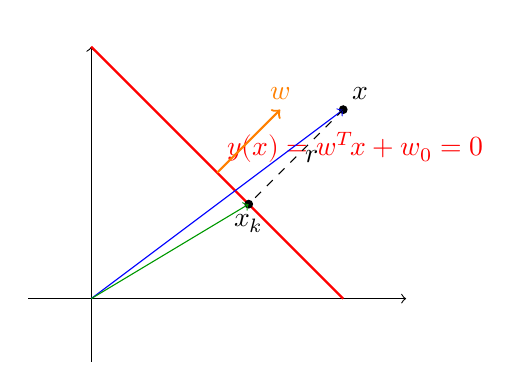
\begin{tikzpicture}[scale=0.8]
        % Axes
        \draw[->] (-1,0) -- (5,0) node[right] {};
        \draw[->] (0,-1) -- (0,4) node[above] {};
        
        % Hyperplane line
        \draw[thick, red] (4,0) -- (0,4) node[midway, above right] {$y(x) = w^T x + w_0 = 0$};
        
        % Point x
        \coordinate (X) at (4, 3);
        \fill (X) circle (2pt) node[above right] {$x$};
        
        % Vector x
        \draw[->, blue] (0,0) -- (X);
        
        % Projection x_p (or x_k) on line
        \coordinate (Xp) at (2.5, 1.5);
        \fill (Xp) circle (2pt) node[below] {$x_k$};
        
        % Vector x_p
        \draw[->, green!60!black] (0,0) -- (Xp);
        
        % Distance r
        \draw[dashed] (X) -- (Xp) node[midway, right] {$r$};
        
        % Weight vector w orthogonal to line
        \draw[->, thick, orange] (2,2) -- (3,3) node[above] {$w$};
    \end{tikzpicture}
    \end{center}
\end{question}

\begin{answer}
\textit{(Πηγή: Lecture 5, slides 12--15)}
    
    \textbf{Γεωμετρική Ερμηνεία:} Η τιμή $y(x)$ εκφράζει την \textbf{προσημασμένη απόσταση} του σημείου $x$ από το υπερεπίπεδο απόφασης, πολλαπλασιασμένη με το μέτρο του διανύσματος βαρών $||w||$.
    
    \textbf{Απόδειξη:} Έστω $x_k$ η κάθετη προβολή του $x$ στο υπερεπίπεδο και $r$ η απόσταση μεταξύ τους:
    $$ x = x_k + r \frac{w}{||w||} $$
    
    Αντικαθιστώντας στη συνάρτηση:
    $$ w^T x = w^T \left(x_k + r \frac{w}{||w||}\right) = w^T x_k + r \frac{||w||^2}{||w||} = w^T x_k + r ||w|| $$
    
    Προσθέτοντας το bias $b$ και χρησιμοποιώντας ότι $w^T x_k + b = 0$ (αφού $x_k$ ανήκει στο υπερεπίπεδο):
    $$ y(x) = w^T x + b = r ||w|| \Rightarrow \boxed{r = \frac{y(x)}{||w||}} $$
\end{answer}

\begin{question}[Θέμα 1.2]
\textbf{Τι είναι τα διανύσματα στήριξης (support vectors) και ποια η σημασία τους;}
\end{question}

\begin{answer}
\textit{(Πηγή: Lecture 6, slides 52--53)}
    
    Τα \textbf{Support Vectors} είναι τα σημεία εκπαίδευσης που βρίσκονται ακριβώς πάνω στα περιθώρια (margins) του ταξινομητή SVM, δηλαδή ικανοποιούν $y_i(w^T x_i + b) = 1$.
    
    \textbf{Σημασία:}
    \begin{itemize}
        \item 
Ορίζουν πλήρως το όριο απόφασης --- η αφαίρεση μη-SVs δεν αλλάζει τον ταξινομητή
        \item Καθορίζουν το πλάτος του margin: $\text{margin} = \frac{2}{||w||}$
        \item Η λύση εξαρτάται \textbf{μόνο} από αυτά (sparse solution)
        \item Είναι τα "δύσκολα" σημεία που βρίσκονται κοντά στο σύνορο των κλάσεων
    \end{itemize}
\end{answer}

\begin{question}[Θέμα 1.3]
\textbf{Πώς αντιμετωπίζουμε το πρόβλημα των μη γραμμικά διαχωρίσιμων κλάσεων με τη χρήση των SVM;}
\end{question}

\begin{answer}
\textit{(Πηγή: Lecture 6, slides 78--79)}
    
    Χρησιμοποιούμε το \textbf{Kernel Trick}: αντί να υπολογίζουμε ρητά τον μετασχηματισμό $\phi(x)$ σε χώρο υψηλότερης διάστασης, χρησιμοποιούμε μια συνάρτηση kernel $K(x, x') = \phi(x)^T \phi(x')$ που υπολογίζει απευθείας το εσωτερικό γινόμενο.
    
    \textbf{Δημοφιλή Kernels:}
    \begin{itemize}
        \item 
\textbf{Πολυωνυμικό:} $K(x, x') = (x^T x' + c)^d$
        \item \textbf{RBF (Gaussian):} $K(x, x') = \exp\left(-\frac{||x - x'||^2}{2\sigma^2}\right)$
    \end{itemize}
    
    Στο νέο χώρο τα δεδομένα είναι συχνά γραμμικά διαχωρίσιμα.
\end{answer}

\begin{question}[Θέμα 1.4]
\textbf{Περιγράψτε τη διαδικασία εφαρμογής της ταξινόμησης κατά Bayes (Risk minimization).}
\end{question}

\begin{answer}
\textit{(Πηγή: Lecture 3, slides 22--24)}
    
\textbf{Βήματα:}
\begin{enumerate}
    \item Ορίζουμε τη \textbf{συνάρτηση απώλειας} $\lambda(\alpha_i|\omega_j)$: το κόστος της απόφασης $\alpha_i$ όταν η πραγματική κλάση είναι $\omega_j$
    \item Υπολογίζουμε το \textbf{υπό συνθήκη ρίσκο}: $R(\alpha_i|x) = \sum_{j=1}^{c} \lambda(\alpha_i|\omega_j) P(\omega_j|x)$
    \item Επιλέγουμε την ενέργεια που \textbf{ελαχιστοποιεί} το ρίσκο: $\alpha^* = \arg\min_i R(\alpha_i|x)$
\end{enumerate}

Για 0-1 loss ($\lambda = 0$ αν σωστό, $\lambda = 1$ αν λάθος), ο κανόνας Bayes επιλέγει την κλάση με τη μέγιστη a posteriori πιθανότητα (\textbf{MAP}).
\end{answer}

\begin{question}[Θέμα 1.5]
\textbf{Περιγράψτε τη βασική ιδέα EM για Mixture of Gaussians.}
\end{question}

\begin{answer}
\textit{(Πηγή: Lecture 9-10, slides 31--36)}
    
Ο αλγόριθμος \textbf{Expectation-Maximization (EM)} χρησιμοποιείται όταν έχουμε λανθάνουσες (hidden) μεταβλητές. Για Gaussian Mixture Models (GMM):

\textbf{E-Step:} Υπολογίζουμε τις "responsibilities" --- την πιθανότητα κάθε σημείο να ανήκει σε κάθε component:
$$ \gamma_{nk} = \frac{\pi_k \mathcal{N}(x_n|\mu_k, \Sigma_k)}{\sum_{j=1}^{K} \pi_j \mathcal{N}(x_n|\mu_j, \Sigma_j)} $$

\textbf{M-Step:} Ενημερώνουμε τις παραμέτρους με βάση τις responsibilities:
\begin{itemize}
    \item $\mu_k^{\text{new}} = \frac{\sum_n \gamma_{nk} x_n}{\sum_n \gamma_{nk}}$ (σταθμισμένος μέσος)
    \item $\Sigma_k^{\text{new}} = $ σταθμισμένη συνδιακύμανση
    \item $\pi_k^{\text{new}} = \frac{1}{N}\sum_n \gamma_{nk}$ (mixing proportion)
\end{itemize}

Επαναλαμβάνουμε μέχρι σύγκλιση. Ο EM \textbf{εγγυάται} αύξηση της log-likelihood σε κάθε βήμα.
\end{answer}

\begin{question}[Θέμα 2.1]
\textbf{Η σύγκλιση του EM εξαρτάται από το learning rate.} \\
\end{question}

\begin{answer}
\textit{(Πηγή: Lecture 9-10, slides 31--36)}

\textbf{Απ: Λάθος.}

Ο EM \textbf{δεν} χρησιμοποιεί learning rate. Είναι αλγόριθμος \textbf{coordinate ascent} που εναλλάσσεται μεταξύ E-step και M-step με κλειστές εκφράσεις. Η σύγκλιση εξαρτάται από την αρχικοποίηση, όχι από learning rate.
\end{answer}

\begin{question}[Θέμα 2.2]
\textbf{Το όριο απόφασης Gaussian classifiers είναι πάντα γραμμικό.} \\
\end{question}

\begin{answer}
    \textit{(Πηγή: Lecture 3, slides 41--42)}

    \textbf{Απ: Λάθος.}
    
    Το όριο απόφασης είναι γραμμικό \textbf{μόνο} όταν οι πίνακες συνδιακύμανσης είναι ίσοι ($\Sigma_1 = \Sigma_2$). Διαφορετικά, ο διακριτικός λόγος περιέχει τετραγωνικούς όρους $x^T(\Sigma_1^{-1} - \Sigma_2^{-1})x$, οπότε το όριο είναι \textbf{τετραγωνικό} (ελλειπτικές/υπερβολικές καμπύλες).
\end{answer}

\begin{question}[Θέμα 2.3]
\textbf{H $k(x, y) = x_1^2 y_1^2 + x_2^2 y_2^2$ είναι kernel.} \\
\end{question}

\begin{answer}
    \textit{(Πηγή: Lecture 6, slide 76)}

    \textbf{Απ: Σωστό.}
    
    Ναι, γιατί μπορεί να γραφτεί ως εσωτερικό γινόμενο:
    $$ k(x, y) = \Phi(x)^T \Phi(y) \text{ όπου } \Phi(x) = [x_1^2, x_2^2]^T $$
    
    Εναλλακτικά, ο πίνακας Gram είναι θετικά ημι-ορισμένος (αφού είναι άθροισμα θετικών kernels).
\end{answer}

\begin{question}[Θέμα 2.4]
\textbf{H διάσταση του feature space ενός kernel μπορεί να είναι άπειρη.} \\
\end{question}

\begin{answer}
    \textit{(Πηγή: Lecture 6, slide 78)}

    \textbf{Απ: Σωστό.}
    
    Το \textbf{RBF kernel} $K(x, x') = e^{-\gamma||x-x'||^2}$ αντιστοιχεί σε άπειρης διάστασης feature space. Η Taylor expansion του $e^x$ δίνει άπειρους όρους, καθένας από τους οποίους αντιστοιχεί σε ένα feature.
\end{answer}

\begin{question}[Θέμα 2.5]
\textbf{Τα PCA components είναι ιδιοδιανύσματα του data matrix.} \\
\end{question}

\begin{answer}
    \textit{(Πηγή: Lecture 9-10, slides 52--54)}

    \textbf{Απ: Λάθος.}
    
    Τα principal components είναι τα \textbf{ιδιοδιανύσματα του πίνακα συνδιακύμανσης} $\Sigma = \frac{1}{N}X^T X$ (αν τα δεδομένα είναι κεντραρισμένα), \textbf{όχι} του data matrix $X$.
    
    Η σχέση μέσω SVD: αν $X = U \Sigma V^T$, τα PCs είναι οι στήλες του $V$.
\end{answer}







\begin{question}[Θέμα 3.1]
Θέλετε να εκπαιδεύσετε ένα Νευρωνικό Δίκτυο (ΝΝ) για αυτόνομη οδήγηση. Τα δεδομένα εκπαίδευσης αποτελούνται από grayscale εικόνες $64 \times 64$ εικονοστοιχείων (pixels). Οι ετικέτες (labels) που συνοδεύουν τα δεδομένα σας είναι η γωνία του τιμονιού σε μοίρες και η ταχύτητα σε χλμ/ώρα (διάνυσμα $y$). Το ΝΝ αποτελείται από ένα στρώμα εισόδου (input layer), από ένα κρυφό στρώμα (hidden layer) 2048 νευρώνων, κι ένα στρώμα εξόδου (output layer).
\end{question}

\begin{answer}
\textit{(Πηγή: Lecture 7, slides 1--2)}
    
    Κάθε στρώμα έχει: (αριθμός εισόδων + 1 bias) $\times$ αριθμός νευρώνων
    
    \begin{itemize}
        \item 
\textbf{Layer 1 (Input → Hidden):} $(4096 + 1) \times 2048 = 8,390,656$ παράμετροι
        \item \textbf{Layer 2 (Hidden → Output):} $(2048 + 1) \times 2 = 4,098$ παράμετροι
    \end{itemize}
    
    \textbf{Σύνολο:} $8,390,656 + 4,098 = \mathbf{8,394,754}$ παράμετροι
\end{answer}

\begin{question}[Θέμα 3.2]
Αν η έξοδος του ΝΝ είναι $z$, η έξοδος του κρυφού στρώματος είναι $h$ και ο πίνακας βαρών μεταξύ κρυφού στρώματος και στρώματος εξόδου είναι $W$, βρείτε την παράγωγο $\frac{\partial J}{\partial W_{ij}}$ αν $J = \frac{1}{2} \|z - y\|^2$ είναι η συνάρτηση κόστους. (2 μονάδες)
\end{question}

\begin{answer}
\textit{(Πηγή: Lecture 7, slides 55--59)}
    
    Για MSE loss: $J = \frac{1}{2} ||z - y||^2$ όπου $z = Wh$ (έξοδος δικτύου)
    
    Εφαρμόζοντας chain rule:
    $$ \frac{\partial J}{\partial W_{ij}} = \frac{\partial J}{\partial z_i} \cdot \frac{\partial z_i}{\partial W_{ij}} = (z_i - y_i) \cdot h_j $$
    
    Σε μορφή πίνακα: $\nabla_W J = (z - y) h^T$ (outer product)
\end{answer}


% ==========================================
% ΙΟΥΝΙΟΣ 2023
% ==========================================


\clearpage
\section{Ιούνιος 2023}

\textit{Πτυχιακή Εξεταστική - 27 Ιουνίου 2023}

\textit{Στις παρακάτω προτάσεις κυκλώστε \textbf{Σ} αν η πρόταση είναι Σωστή και \textbf{Λ} αν η πρόταση είναι Λανθασμένη. Κάθε σωστή απάντηση λαμβάνει 1 μονάδα και κάθε λάθος απάντηση λαμβάνει -0.25.}





\begin{question}[Θέμα 1.1]
\textbf{Η αντικειμενική συνάρτηση (objective function) ενός τεχνητού νευρωνικού δικτύου (ΤΝΔ) μπορεί έχει τοπικά ακρότατα.}
\end{question}

\begin{answer}
    \textit{(Πηγή: Lecture 7, slides 57--58)}
    \textbf{Απ: Σωστό.} 
    \textit{Εξήγηση:} Η συνάρτηση κόστους των νευρωνικών δικτύων είναι \textbf{μη-κυρτή (non-convex)}. Λόγω των συμμετριών στα βάρη (permutation symmetry) και των μη-γραμμικοτήτων, δημιουργούνται πολλαπλά τοπικά ελάχιστα (local minima) και σαγματικά σημεία (saddle points). Δεν εγγυάται η εύρεση του ολικού ελαχίστου.
\end{answer}

\begin{question}[Θέμα 1.2]
\textbf{Η αντικειμενική συνάρτηση (objective function) ενός SVM μπορεί έχει τοπικά ακρότατα.}
\end{question}

\begin{answer}
    \textit{(Πηγή: Lecture 6, slides 44--47)}
    \textbf{Απ: Λάθος.} 
    \textit{Εξήγηση:} Το πρόβλημα βελτιστοποίησης των SVM είναι πρόβλημα \textbf{κυρτού τετραγωνικού προγραμματισμού} (Convex Quadratic Programming). Η αντικειμενική συνάρτηση $J(w) = \frac{1}{2}||w||^2 + C \sum \xi_i$ είναι κυρτή και οι περιορισμοί είναι γραμμικοί. Συνεπώς, κάθε τοπικό ελάχιστο είναι και \textbf{ολικό (global minimum)}.
\end{answer}

\begin{question}[Θέμα 1.3]
\textbf{Ο EM αλγόριθμος ελαχιστοποιεί την συνάρτηση πιθανοφάνειας.}
\end{question}

\begin{answer}
    \textit{(Πηγή: Lecture 9-10, slides 31--36)}
    \textbf{Απ: Λάθος.} 
    \textit{Εξήγηση:} Ο αλγόριθμος Expectation-Maximization (EM) στοχεύει στη \textbf{μεγιστοποίηση} της πιθανοφάνειας (Likelihood Maximization). Σε κάθε επανάληψη, υπολογίζει ένα 'lower bound' της log-likelihood και το μεγιστοποιεί, εγγυώμενος ότι η πιθανοφάνεια δεν θα μειωθεί.
\end{answer}

\begin{question}[Θέμα 1.4]
\textbf{Η αντικειμενική συνάρτηση ενός ΤΝΔ που εκπαιδεύεται με gradient descent σταματά να μειώνεται μετά από πεπερασμένο αριθμό επαναλήψεων εκπαίδευσης.}
\end{question}

\begin{answer}
    \textit{(Πηγή: Lecture 7, slides 59--61)}
    \textbf{Απ: Λάθος.} 
    \textit{Εξήγηση:} Η σύγκλιση της Gradient Descent είναι θεωρητικά \textbf{ασυμπτωτική}. Καθώς πλησιάζουμε το ελάχιστο, η κλίση (gradient) τείνει στο μηδέν, κάνοντας τα βήματα ενημέρωσης ολοένα και μικρότερα. Θεωρητικά, μπορεί να απαιτηθούν άπειρα βήματα για να φτάσουμε \textit{ακριβώς} στο ελάχιστο (αν και πρακτικά σταματάμε όταν η αλλαγή είναι μικρότερη από ένα κατώφλι ανοχής).
\end{answer}

\begin{question}[Θέμα 1.5]
\textbf{Ένα γραμμικό SVM εκπαιδεύεται με το παρακάτω σύνολο δεδομένων, όπου $x_i$ είναι τα δεδομένα και $d$ η επιθυμητή ταξινόμηση κάθε διανύσματος.}
    
    \begin{table}[H]
        \centering
        \begin{tabular}{|c|c|c||c|c|c|}
        \hline
        $x_1$ & $x_2$ & $d$ & $x_1$ & $x_2$ & $d$ \\ \hline
        -2    & 7     & -1  & 1     & 0     & +1  \\ \hline
        2     & 6     & -1  & 6     & 6     & +1  \\ \hline
        4     & 12    & -1  & 6     & 10    & +1  \\ \hline
        \end{tabular}
    \end{table}

    \textbf{Η νέα είσοδος (4,3) στο παραπάνω γραμμικό SVM θα ταξινομηθεί ως κλάση -1.}
\end{question}

\begin{answer}
    \textit{(Πηγή: Lecture 6, slides 49--55)}
    \textbf{Απ: Λάθος.} (Ταξινομείται ως +1)
    
    \textbf{Αναλυτική Επίλυση -- Εύρεση Διαχωριστικής Ευθείας:}
    
    \textbf{Βήμα 1: Εντοπισμός Support Vectors.}
    Τα SVs είναι τα σημεία πιο κοντά στο σύνορο:
    \begin{itemize}
        \item Κλάση +1: $(1, 0)$ και $(6, 10)$
        \item Κλάση -1: $(2, 6)$
    \end{itemize}
    
    \textbf{Βήμα 2: Υπολογισμός κλίσης.}
    Η ευθεία που συνδέει τα SVs της κλάσης +1:
    $$ \text{slope} = \frac{10 - 0}{6 - 1} = \frac{10}{5} = 2 $$
    
    \textbf{Βήμα 3: Εύρεση margin boundaries.}
    Μορφή: $x_2 = 2x_1 + b$
    
    \underline{Margin +1} (περνάει από $(1,0)$):
    $0 = 2(1) + b_+ \Rightarrow b_+ = -2 \Rightarrow x_2 = 2x_1 - 2$
    
    \underline{Margin -1} (περνάει από $(2,6)$):
    $6 = 2(2) + b_- \Rightarrow b_- = 2 \Rightarrow x_2 = 2x_1 + 2$
    
    \textbf{Βήμα 4: Decision Boundary (μέση ευθεία).}
    $$ b = \frac{-2 + 2}{2} = 0 \Rightarrow \boxed{x_2 = 2x_1} \quad \text{ή} \quad 2x_1 - x_2 = 0 $$
    
    \textbf{Βήμα 5: Ταξινόμηση.}
    Κανόνας: $y(x) = 2x_1 - x_2$. Αν $y > 0 \Rightarrow +1$, αν $y < 0 \Rightarrow -1$.
    
    \begin{tabular}{|c|c|c|}
    \hline
    Σημείο & $y = 2x_1 - x_2$ & Κλάση \\ \hline
    $(4, 3)$ & $2(4) - 3 = 5 > 0$ & \textbf{+1} \\ \hline
    $(0, 4)$ & $2(0) - 4 = -4 < 0$ & \textbf{-1} \\ \hline
    $(3, 7)$ & $2(3) - 7 = -1 < 0$ & \textbf{-1} \\ \hline
    \end{tabular}
\end{answer}

\begin{question}[Θέμα 1.6]
\textbf{Η νέα είσοδος (0,4) στο παραπάνω γραμμικό SVM θα ταξινομηθεί ως κλάση -1.}
\end{question}

\begin{answer}
    \textit{(Πηγή: Lecture 6, slides 49--55)}
    \textbf{Απ: Σωστό.}
\end{answer}

\begin{question}[Θέμα 1.7]
\textbf{Η νέα είσοδος (3,7) στο παραπάνω γραμμικό SVM θα ταξινομηθεί ως κλάση +1.}
\end{question}

\begin{answer}
    \textit{(Πηγή: Lecture 6, slides 49--55)}
    \textbf{Απ: Λάθος.} (Ταξινομείται ως -1)

    \begin{center}
    \begin{tikzpicture}[scale=0.6]
        % Axes
        \draw[->] (-3,0) -- (8,0) node[right] {$x_1$};
        \draw[->] (0,-1) -- (0,13) node[above] {$x_2$};


        
        % Data Points (-1)
        \fill[red] (-2,7) circle (3pt) node[left] {-1};
        \fill[red] (2,6) circle (3pt) node[below] {-1};
        \fill[red] (4,12) circle (3pt) node[above] {-1};
        
        % Data Points (+1)
        \fill[blue] (1,0) circle (3pt) node[below] {+1};
        \fill[blue] (6,6) circle (3pt) node[right] {+1};
        \fill[blue] (6,10) circle (3pt) node[right] {+1};
        
        % Test Points
        \draw[thick, orange] (4,3) circle (3pt) node[below] {(4,3)};
        \draw[thick, orange] (0,4) circle (3pt) node[left] {(0,4)};
        \draw[thick, orange] (3,7) circle (3pt) node[above] {(3,7)};
        
        % Decision Boundary
        % Decision Boundary (Exact Calculation)
        % Support Vectors: Class -1: (2,6). Class +1: (1,0) and (6,10).
        % Line connecting (+1) SVs (1,0) and (6,10) has slope (10-0)/(6-1) = 2.
        % Boundary is parallel to this, slope 2. Form x2 = 2*x1 + b.
        % Margin boundaries:
        % Through (1,0): 0 = 2(1) + b+ -> b+ = -2. (x2 = 2x1 - 2)
        % Through (2,6): 6 = 2(2) + b- -> b- = 2.  (x2 = 2x1 + 2)
        % Decision Boundary is midline: b = (-2+2)/2 = 0. -> x2 = 2x1.
        \draw[dashed, thick] (-0.5,-1) -- (6.5,13) node[right] {$x_2 = 2x_1$};
        \draw[dotted, gray] (0,-2) -- (7,12); % Margin +1 (x2 = 2x1 - 2)
        \draw[dotted, gray] (-1,0) -- (5.5,13); % Margin -1 (x2 = 2x1 + 2)
    \end{tikzpicture}
    \end{center}
\end{answer}

\begin{question}[Θέμα 1.8]
\textbf{Η αντικειμενική συνάρτηση του k-Means αλγορίθμου σταματά να μειώνεται μετά από πεπερασμένο αριθμό επαναλήψεων εκπαίδευσης.}
\end{question}

\begin{answer}
    \textit{(Πηγή: Lecture 9-10, slide 10)}
    \textbf{Απ: Σωστό.} 
    \textit{Εξήγηση:} Ο αλγόριθμος K-Means εγγυάται σύγκλιση σε πεπερασμένο αριθμό βημάτων επειδή:
    \begin{enumerate}
        \item Υπάρχει πεπερασμένος αριθμός τρόπων ανάθεσης $N$ σημείων σε $K$ clusters ($K^N$).
        \item Σε κάθε βήμα, η συνάρτηση κόστους (sum of squared errors) μειώνεται μονοτονικά ή παραμένει σταθερή.
        \item Δεν υπάρχουν κύκλοι (loops) στις αναθέσεις.
    \end{enumerate}
\end{answer}

\begin{question}[Θέμα 1.9]
\textbf{Η βέλτιστη τιμή της αντικειμενικής συνάρτησης ενός EM αλγορίθμου (για την εκτίμηση μιας πυκνότητας πιθανότητας) χρησιμοποιώντας $p+1$ γκαουσιανές συναρτήσεις \underline{δεν} μπορεί να είναι υψηλότερη από αυτήν της αντικειμενικής συνάρτησης για την εκτίμηση της ίδιας πυκνότητας πιθανότητας χρησιμοποιώντας $p$ γκαουσιανές συναρτήσεις.}
\end{question}

\begin{answer}
    \textit{(Πηγή: Lecture 9-10, slides 31--36)}
    \textbf{Απ: Λάθος.} 
    \textit{Εξήγηση:} Όταν αυξάνουμε την πολυπλοκότητα του μοντέλου (π.χ. από $p$ σε $p+1$ Gaussians), το νέο μοντέλο περιέχει το παλιό ως ειδική περίπτωση (nested models). Συνεπώς, η μέγιστη πιθανοφάνεια (likelihood) του $p+1$ μοντέλου θα είναι \textbf{τουλάχιστον ίση ή μεγαλύτερη} από αυτή του $p$ μοντέλου. (Προσοχή: Αυτό μπορεί να οδηγήσει σε overfitting, αλλά η likelihood στο training set αυξάνεται).
\end{answer}

\begin{question}[Θέμα 1.10]
\textbf{Στα ΤΝΔ οι συναρτήσεις ενεργοποίησης (activation functions) βοηθούν ώστε να σχηματιστούν μη γραμμικά όρια απόφασης (decision boundaries).}
\end{question}

\begin{answer}
    \textit{(Πηγή: Lecture 7, slides 28--30)}
    \textbf{Απ: Σωστό.} 
    \textit{Εξήγηση:} Μια σύνθεση γραμμικών συναρτήσεων είναι απλά μια άλλη γραμμική συνάρτηση ($W_2(W_1 x) = W' x$). Χωρίς μη-γραμμικές συναρτήσεις ενεργοποίησης (όπως ReLU, Sigmoid, Tanh), ένα πολυεπίπεδο νευρωνικό δίκτυο καταρρέει σε ένα απλό γραμμικό μοντέλο (Perceptron), χάνοντας την ικανότητα να προσεγγίζει πολύπλοκες, μη-γραμμικές συναρτήσεις (Universal Approximation Theorem).
\end{answer}


% ==========================================
% ΣΕΠΤΕΜΒΡΙΟΣ 2023
% ==========================================


\clearpage
\section{Σεπτέμβριος 2023}

\textit{Εξεταστική Σεπτεμβρίου - 14 Σεπτεμβρίου 2023}





\begin{question}[Θέμα 1.1]
Υποθέστε ότι έχετε συμπτώματα COVID-19 και αποφασίζετε να κάνετε ένα COVID-test. Στη συσκευασία του test αναγράφεται ότι η πιθανότητα το αποτέλεσμα του test να είναι θετικό δεδομένου ότι άτομο έχει όντως μολυνθεί από τον ιό είναι $0.875$ και ότι η πιθανότητα το αποτέλεσμα του test να είναι αρνητικό δεδομένου ότι το άτομο \textbf{δεν} έχει μολυνθεί από τον ιό είναι $0.975$. Το test που κάνατε βγαίνει θετικό. Υπολογίστε την πιθανότητα να έχετε όντως μολυνθεί από τον ιό με βάση το αποτέλεσμα του test αν η συχνότητα μόλυνσης από τον ιό στην περιοχή που κατοικείτε είναι 1 στους 10.
\end{question}

\begin{answer}
\textit{(Πηγή: Lecture 3, slides 22--24)}
Ορίζουμε τα ενδεχόμενα:
\begin{itemize}
    \item 
$\omega_1$: Δεν έχω μολυνθεί (Υγιής)
    \item $\omega_2$: Έχω μολυνθεί (Ασθενής)
    \item $x=1$: Test Θετικό
    \item $x=0$: Test Αρνητικό
\end{itemize}

Δεδομένα από την εκφώνηση:
\begin{itemize}
    \item $P(x=1 | \omega_2) = 0.875$ (Sensitivity)
    \item $P(x=0 | \omega_1) = 0.975 \Rightarrow P(x=1 | \omega_1) = 0.025$ (False Positive Rate)
    \item $P(\omega_2) = 0.1$, $P(\omega_1) = 0.9$
\end{itemize}

Από το \textbf{θεώρημα Bayes}:
$$ P(\omega_2 | x=1) = \frac{P(x=1 | \omega_2) P(\omega_2)}{P(x=1)} $$

Όπου: $P(x=1) = P(x=1|\omega_1)P(\omega_1) + P(x=1|\omega_2)P(\omega_2) = (0.025 \cdot 0.9) + (0.875 \cdot 0.1) = 0.11$

$$ P(\omega_2 | x=1) = \frac{0.875 \cdot 0.1}{0.11} = \frac{0.0875}{0.11} \approx \mathbf{0.795} \text{ ή } \mathbf{79.5\%} $$
\end{answer}



Θεωρήστε το παρακάτω νευρωνικό δίκτυο (αρχιτεκτονική $3 \to 5 \to 3 \to 2$):

\begin{center}
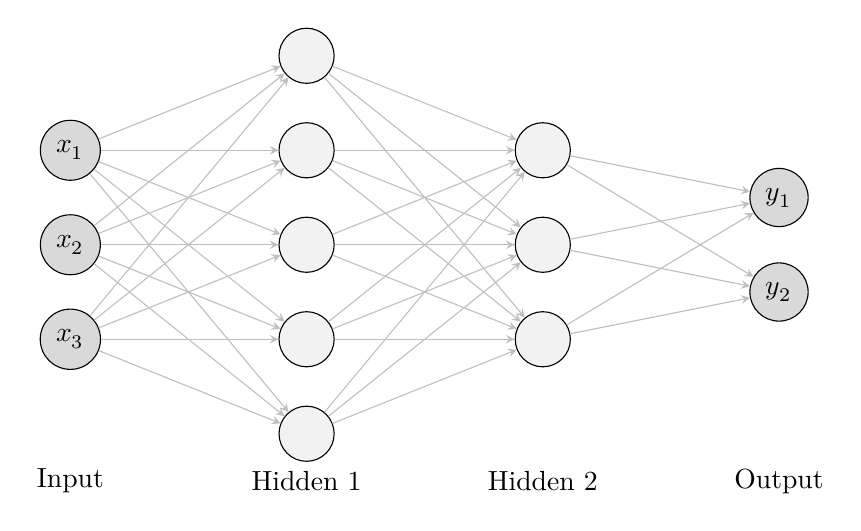
\begin{tikzpicture}[x=1.5cm, y=1.2cm, >=stealth]
% Input Layer
\foreach \m [count=\y] in {1,2,3}
  \node [circle, draw, fill=gray!30, minimum size=0.7cm] (input-\m) at (0, 2.5-\y) {$x_{\y}$};

% Hidden Layer 1 (5 neurons)
\foreach \m [count=\y] in {1,2,3,4,5}
  \node [circle, draw, fill=gray!10, minimum size=0.7cm] (hidden1-\m) at (2, 3.5-\y) {};

% Hidden Layer 2 (3 neurons)
\foreach \m [count=\y] in {1,2,3}
  \node [circle, draw, fill=gray!10, minimum size=0.7cm] (hidden2-\m) at (4, 2.5-\y) {};

% Output Layer (2 neurons)
\foreach \m [count=\y] in {1,2}
  \node [circle, draw, fill=gray!30, minimum size=0.7cm] (output-\m) at (6, 2-\y) {$y_{\y}$};

% Connections
\foreach \i in {1,...,3}
  \foreach \j in {1,...,5}
    \draw [->, gray!50] (input-\i) -- (hidden1-\j);

\foreach \i in {1,...,5}
  \foreach \j in {1,...,3}
    \draw [->, gray!50] (hidden1-\i) -- (hidden2-\j);

\foreach \i in {1,...,3}
  \foreach \j in {1,...,2}
    \draw [->, gray!50] (hidden2-\i) -- (output-\j);

% Labels
\node at (0, -2) {Input};
\node at (2, -2) {Hidden 1};
\node at (4, -2) {Hidden 2};
\node at (6, -2) {Output};
\end{tikzpicture}
\end{center}

\begin{question}[Θέμα 2.1]
\textbf{Βρείτε τις διαστάσεις των πινάκων βαρών, $W^{[1]}, W^{[2]}, W^{[3]}$ και των διανυσμάτων πόλωσης (bias) $b^{[1]}, b^{[2]}, b^{[3]}$. Δώστε τις σε μορφή (αριθμός γραμμών) $\times$ (αριθμός στηλών). (1 μονάδα)}
\end{question}

\begin{answer}
    \textit{(Πηγή: Lecture 7, slides 1--2)}

    \textbf{Γενικός Κανόνας:} Αν το επίπεδο $l-1$ έχει $n_{in}$ νευρώνες και το επίπεδο $l$ έχει $n_{out}$ νευρώνες:
    \begin{itemize}
        \item Ο πίνακας βαρών $W^{[l]}$ έχει διαστάσεις $n_{out} \times n_{in}$.
        \item Το διάνυσμα bias $b^{[l]}$ έχει διαστάσεις $n_{out} \times 1$.
    \end{itemize}

    \textbf{Εφαρμογή:}
    \begin{itemize}
        \item \textbf{Layer 1 ($3 \to 5$):} $n_{in}=3, n_{out}=5 \Rightarrow W^{[1]} \in \mathbb{R}^{5 \times 3}, b^{[1]} \in \mathbb{R}^{5 \times 1}$
        \item \textbf{Layer 2 ($5 \to 3$):} $n_{in}=5, n_{out}=3 \Rightarrow W^{[2]} \in \mathbb{R}^{3 \times 5}, b^{[2]} \in \mathbb{R}^{3 \times 1}$
        \item \textbf{Layer 3 ($3 \to 2$):} $n_{in}=3, n_{out}=2 \Rightarrow W^{[3]} \in \mathbb{R}^{2 \times 3}, b^{[3]} \in \mathbb{R}^{2 \times 1}$
    \end{itemize}
\end{answer}

\begin{question}[Θέμα 2.2]
\textbf{Δώστε τις εξισώσεις της 'προς τα εμπρός διέλευσης' (forward pass) του παραπάνω δικτύου αν κάθε νευρώνας των κρυφών στρωμάτων (hidden layers) και του στρώματος εξόδου (output layer) έχει συνάρτηση ενεργοποίησης (activation function) $g(.)$, έτσι ώστε $a^{[l]} = g(z^{[l]}), i=1,2,3$. (1 μονάδα)}
\end{question}

\begin{answer}
    \textit{(Πηγή: Lecture 7, slides 1--2)}
    
    Η διαδικασία περιλαμβάνει δύο βήματα για κάθε στρώμα: τον γραμμικό συνδυασμό (linear transform) και την μη-γραμμική ενεργοποίηση (activation).
    
    \textbf{Layer 1 (Input $\to$ Hidden 1):}
    $$ z^{[1]} = W^{[1]} x + b^{[1]} \quad (\text{Linear step}) $$
    $$ a^{[1]} = g(z^{[1]}) \quad (\text{Activation, π.χ. ReLU/Sigmoid}) $$
    
    \textbf{Layer 2 (Hidden 1 $\to$ Hidden 2):}
    $$ z^{[2]} = W^{[2]} a^{[1]} + b^{[2]} $$
    $$ a^{[2]} = g(z^{[2]}) $$
    
    \textbf{Layer 3 (Hidden 2 $\to$ Output):}
    $$ z^{[3]} = W^{[3]} a^{[2]} + b^{[3]} $$
    $$ y = a^{[3]} = g(z^{[3]}) \quad (\text{Τελική πρόβλεψη}) $$
    
    όπου $g(\cdot)$ είναι η συνάρτηση ενεργοποίησης (activation function) που εφαρμόζεται κατά στοιχείο (element-wise).
\end{answer}

\begin{question}[Θέμα 2.3]
\textbf{Υπολογίστε τον αριθμό των παραμέτρων εκπαίδευσης. (1 μονάδα)}
\end{question}

\begin{answer}
    \textit{(Πηγή: Lecture 7, slides 1--2)}
    
    Ο συνολικός αριθμός παραμέτρων είναι το άθροισμα των βαρών και των biases σε κάθε επίπεδο.
    Για κάθε επίπεδο: $Params = (n_{in} \times n_{out}) + n_{out} = (n_{in} + 1) \times n_{out}$.
    
    \begin{itemize}
        \item \textbf{Layer 1 ($3 \to 5$):} $(3 \times 5) + 5 = 15 + 5 = 20$
        \item \textbf{Layer 2 ($5 \to 3$):} $(5 \times 3) + 3 = 15 + 3 = 18$
        \item \textbf{Layer 3 ($3 \to 2$):} $(3 \times 2) + 2 = 6 + 2 = 8$
    \end{itemize}
    
    \textbf{Σύνολο:} $20 + 18 + 8 = \mathbf{46}$ παράμετροι.
\end{answer}


\begin{question}[Θέμα 3.1]
Εφαρμόστε για μία επανάληψη τη μέθοδο βελτιστοποίησης gradient descent αν δίνονται το διάνυσμα χαρακτηριστικών $X = [1, 1, 1]^T$, το διάνυσμα των παραμέτρων $W = [1, 1, 1]^T$, η τιμή πόλωσης (bias) $b = 1/2$ και η τιμή στόχου $y = 1.5$ χρησιμοποιώντας σαν συνάρτηση βελτιστοποίησης την συνάρτηση ελαχίστων τετραγώνων. Υποθέστε ρυθμό μάθησης (learning rate) $\eta = 0.1$.
\end{question}

\begin{answer}
    \textit{(Πηγή: Lecture 7, slides 59--61)}

\textbf{Πριν την επανάληψη:}
$$ \hat{y} = W^T X + b = (1+1+1) + 0.5 = 3.5 $$
$$ E_{old} = \frac{1}{2} (3.5 - 1.5)^2 = \frac{1}{2} \cdot 4 = \mathbf{2} $$

\textbf{Gradient Descent Update:}
    Η παράγωγος του σφάλματος ως προς τα βάρη υπολογίζεται με τον κανόνα της αλυσίδας (Chain Rule):
    $$ \frac{\partial E}{\partial W} = \frac{\partial E}{\partial \hat{y}} \cdot \frac{\partial \hat{y}}{\partial W} = (\hat{y} - y) \cdot X $$
    
    Αντικαθιστώντας τις τιμές:
    $$ \frac{\partial E}{\partial W} = (3.5 - 1.5) \cdot [1,1,1]^T = 2 \cdot [1,1,1]^T = [2,2,2]^T $$
    
    Ενημέρωση βαρών ($W_{new} = W - \eta \frac{\partial E}{\partial W}$):
    $$ W_{new} = [1,1,1]^T - 0.1 \cdot [2,2,2]^T = [1,1,1]^T - [0.2, 0.2, 0.2]^T = [0.8, 0.8, 0.8]^T $$
    
    Ενημέρωση bias ($b_{new} = b - \eta \frac{\partial E}{\partial b}$):
    $$ b_{new} = b - \eta (\hat{y} - y) = 0.5 - 0.1 \cdot 2 = 0.3 $$

\textbf{Μετά την επανάληψη:}
$$ \hat{y}_{new} = (0.8+0.8+0.8) + 0.3 = 2.7 $$
$$ E_{new} = \frac{1}{2} (2.7 - 1.5)^2 = \frac{1}{2} \cdot 1.44 = \mathbf{0.72} $$

\textbf{Παρατήρηση:} Το κόστος μειώθηκε από 2 σε 0.72, άρα ο αλγόριθμος λειτουργεί σωστά.
\end{answer}

\begin{question}[Θέμα 3.2]
\textbf{Γιατί επιλέγουμε συνήθως μικρές τιμές για τον ρυθμό μάθησης;}
\end{question}

\begin{answer}
    \textit{(Πηγή: Lecture 7, slide 61)}
    \textbf{Learning Rate ($\eta$):} 
    \begin{itemize}
        \item \textbf{Μικρό $\eta$:} Εξασφαλίζει σταθερή σύγκλιση/μείωση του σφάλματος, αλλά μπορεί να είναι αργή.
        \item \textbf{Μεγάλο $\eta$:} Μπορεί να οδηγήσει σε ταλαντώσεις (oscillations) γύρω από το ελάχιστο ή ακόμη και σε απόκλιση (overshooting), αυξάνοντας το σφάλμα αντί να το μειώνει.
    \end{itemize}
    Συνήθως επιλέγουμε μικρές τιμές (π.χ. $0.1, 0.01$) για ασφάλεια.
\end{answer}

% ==========================================
% ΦΕΒΡΟΥΑΡΙΟΣ 2024
% ==========================================


\clearpage
\section{Φεβρουάριος 2024}

\textit{Εξεταστική Φεβρουαρίου - 14 Φεβρουαρίου 2024}

\textit{Στις παρακάτω προτάσεις κυκλώστε \textbf{όλες} τις πιθανές \textbf{σωστές} απαντήσεις. Κάθε σωστή απάντηση λαμβάνει 0.5 μονάδα και κάθε λάθος απάντηση λαμβάνει -0.25.}





\begin{question}[Θέμα 1.1]
\textbf{Τα Νευρωνικά Δίκτυα:}
    \begin{itemize}
        \item [Α.] Βελτιστοποιούν μια κυρτή (convex) συνάρτηση κόστους
        \item [Β.] Δίνουν πάντα έξοδο 0 ή 1
        \item [Γ.] Μπορούν να χρησιμοποιηθούν τόσο για παλινδρόμηση όσο και για ταξινόμηση
        \item [Δ.] Μπορούν να χρησιμοποιηθούν σε «επίτρεπη» ταξινομητών
    \end{itemize}
\end{question}

\begin{answer}
    \textit{(Πηγή: Lecture 7, slides 57--58)}

    \textbf{Απ: Γ, Δ.}
    
    \textit{Εξήγηση:} Η συνάρτηση κόστους NN δεν είναι κυρτή (Α λάθος). Η έξοδος εξαρτάται από την activation function (Β λάθος). Τα NN χρησιμοποιούνται και για regression και classification (Γ σωστό) και μπορούν να συνδυαστούν σε ensemble (Δ σωστό).
\end{answer}

\begin{question}[Θέμα 1.2]
\textbf{Ποιο/ποια από τα παρακάτω είναι σωστό/σωστά για τα Πιθανοκρατικά Αναγεννητικά Μοντέλα (Probabilistic Generative Models, PGM):}
    \begin{itemize}
        \item [Α.] Μοντελοποιούν την από κοινού συνάρτηση κατανομής $P(\omega_j, x)$
        \item [Β.] Ο Perceptron είναι PGM
        \item [Γ.] Μπορούν να χρησιμοποιηθούν για ταξινόμηση
        \item [Δ.] Η Γραμμική Ανάλυση Διακριτοποίησης (Linear Discriminant Analysis) είναι PGM
    \end{itemize}
\end{question}

\begin{answer}
    \textit{(Πηγή: Lecture 5, slides 70--72)}

    \textbf{Απ: Α, Γ, Δ.}
    
    \textit{Εξήγηση:} PGMs μοντελοποιούν την joint distribution (Α σωστό). Ο Perceptron είναι discriminative (Β λάθος). Χρησιμοποιούνται για classification μέσω Bayes (Γ σωστό). Το LDA είναι generative (Δ σωστό).
\end{answer}

\begin{question}[Θέμα 1.3]
\textbf{Ποιες από τις παρακάτω μεθόδους μπορούν να επιτύχουν μηδενικό σφάλμα ταξινόμησης σε κάθε σύνολο εκπαίδευσης που είναι γραμμικά διαχωρίσιμο;}
    \begin{itemize}
        \item [Α.] Δέντρο απόφασης
        \item [Β.] 15-NN
        \item [Γ.] Hard-Margin SVM
        \item [Δ.] Perceptron
    \end{itemize}
\end{question}

\begin{answer}
    \textit{(Πηγή: Lecture 6, slides 44--47; Lecture 5, slides 26--31)}

    \textbf{Απ: Γ, Δ.}
    
    \textit{Εξήγηση:} Δέντρα δεν εγγυώνται γραμμικό διαχωρισμό. 15-NN μπορεί να κάνει λάθη λόγω voting. Hard-margin SVM βρίσκει τέλειο γραμμικό διαχωρισμό (Γ σωστό). Ο Perceptron συγκλίνει για γραμμικά διαχωρίσιμα δεδομένα (Δ σωστό).
\end{answer}

\begin{question}[Θέμα 1.4]
\textbf{Το kernel trick:}
    \begin{itemize}
        \item [Α.] Μπορεί να εφαρμοστεί σε κάθε αλγόριθμο ταξινόμησης
        \item [Β.] Χρησιμοποιείται συνήθως για μείωση διαστάσεων
        \item [Γ.] Εκμεταλλεύεται το γεγονός ότι σε πολλούς αλγορίθμους τα βάρη μπορούν να γραφούν σαν γραμμικός συνδυασμός των δεδομένων εισόδου
        \item [Δ.] Δίνει πάντα τιμές μεταξύ 0 και 1
    \end{itemize}
\end{question}

\begin{answer}
    \textit{(Πηγή: Lecture 6, slides 78--79)}

    \textbf{Απ: Γ.}
    
    \textit{Εξήγηση:} Το kernel trick βασίζεται στο Representer Theorem (Γ σωστό) --- τα βάρη γράφονται ως $w = \sum_i \alpha_i \phi(x_i)$.
\end{answer}

\begin{question}[Θέμα 1.5]
\textbf{Στα Νευρωνικά Δίκτυα, οι συναρτήσεις ενεργοποίησης ReLU και tanh:}
    \begin{itemize}
        \item [Α.] Βοηθούν στην επιτάχυνση της διαδικασίας εκπαίδευσης
        \item [Β.] Οδηγούν στην εύρεση μη γραμμικών ορίων απόφασης
        \item [Γ.] Εφαρμόζονται μόνο στους νευρώνες του επιπέδου εξόδου (output layer)
        \item [Δ.] Δίνουν πάντα τιμές μεταξύ 0 και 1
    \end{itemize}
\end{question}

\begin{answer}
    \textit{(Πηγή: Lecture 7, slides 28--30)}

    \textbf{Απ: Α, Β.}
    
    \textit{Εξήγηση:} ReLU επιταχύνει training (Α σωστό). Μη-γραμμικές activations επιτρέπουν μη-γραμμικά όρια (Β σωστό). Εφαρμόζονται σε hidden layers (Γ λάθος). ReLU δίνει $[0, \infty)$, tanh δίνει $[-1, 1]$ (Δ λάθος).
\end{answer}

\begin{question}[Θέμα 1.6]
\textbf{Με βάση το Bias-Variance Trade-off ένας 1-NN ταξινομητής έχει \_\_\_\_\_\_\_\_ σε σύγκριση με έναν 3-NN ταξινομητή:}
    \begin{itemize}
        \item [Α.] Μεγαλύτερο variance
        \item [Β.] Μεγαλύτερο bias
        \item [Γ.] Μικρότερο variance
        \item [Δ.] Μικρότερο bias
    \end{itemize}
\end{question}

\begin{answer}
    \textit{(Πηγή: Lecture 2, slides 32--37)}

    \textbf{Απ: Α, Δ.}
    
    \textit{Εξήγηση:} 1-NN: υψηλό variance (ευαίσθητο σε θόρυβο), χαμηλό bias (ακριβές στο training). 3-NN: χαμηλότερο variance (averaging), υψηλότερο bias.
\end{answer}

\begin{question}[Θέμα 1.7]
\textbf{Ποια/α από τα παρακάτω είναι αληθές/ή για το Bootstrapping:}
    \begin{itemize}
        \item [Α.] Με το Bootstrapping επιλέγουμε τυχαία δείγματα από τα δεδομένα με επανατοποθέτηση
        \item [Β.] Σκοπός του είναι να οδηγήσει σε μείωση του bias
        \item [Γ.] Είναι μη αποτελεσματικό με Logistic Regression ταξινομητές
    \end{itemize}
\end{question}

\begin{answer}
    \textit{(Πηγή: Lecture 8, slides 10--12)}

    \textbf{Απ: Α.}
    
    \textit{Εξήγηση:} Bootstrapping = sampling with replacement (Α σωστό). Μειώνει variance, όχι bias (Β λάθος). Λειτουργεί με όλους τους ταξινομητές (Γ λάθος).
\end{answer}

\begin{question}[Θέμα 1.8]
\textbf{Ποια/α από τα παρακάτω είναι αληθές/ή για το PCA:}
    \begin{itemize}
        \item [Α.] Προσθέτοντας ένα '1' στο τέλος κάθε διανύσματος δεδομένων δεν αλλάζουν τα αποτελέσματα του PCA
        \item [Β.] Οι πρωταρχικές συνιστώσες είναι ιδιοδιανύσματα του πίνακα συμμεταβλητότητας των δεδομένων
        \item [Γ.] Οι πρωταρχικές συνιστώσες είναι ιδιοδιανύσματα του πίνακα των δεδομένων
    \end{itemize}
\end{question}

\begin{answer}
    \textit{(Πηγή: Lecture 9-10, slides 52--54)}

    \textbf{Απ: Α, Β.}
    
    \textit{Εξήγηση:} Σταθερό feature δεν αλλάζει variance (Α σωστό). PCs = eigenvectors of covariance matrix (Β σωστό, Γ λάθος).
\end{answer}

\begin{question}[Θέμα 1.9]
\textbf{Ποια/ες από τις παρακάτω προσεγγίσεις μπορούν να βοηθήσουν ώστε να αποφευχθεί το overfitting στα Δέντρα Απόφασης:}
    \begin{itemize}
        \item [Α.] Κλάδεμα (Pruning)
        \item [Β.] Ορισμός μέγιστου βάθους του δέντρου
        \item [Γ.] Ορισμός ελάχιστου αριθμού από δείγματα στα φύλλα
    \end{itemize}
\end{question}

\begin{answer}
    \textit{(Πηγή: Lecture 8, slides 71--72)}

    \textbf{Απ: Α, Β, Γ.}
    
    \textit{Εξήγηση:} Όλες οι τεχνικές περιορίζουν την πολυπλοκότητα του δέντρου και αποφεύγουν overfitting.
\end{answer}

\begin{question}[Θέμα 1.10]
\textbf{Έστω ότι έχετε σετ δεδομένων που αποτελείται από n δείγματα διαφορετικών κλάσεων. Κάθε κλάση έχει διαφορετική κατανομή. Δεν γνωρίζουμε τις ετικέτες των κλάσεων και έτσι χρησιμοποιείτε μια τεχνική ομαδοποίησης (clustering), την k-Means. Σε ποιες από τις παρακάτω περιπτώσεις θα επηρεαζόταν αρνητικά η αποδοτικότητα της μεθόδου:}
    \begin{itemize}
        \item [Α.] Κάποιες από τις κλάσεις δεν ακολουθούν κανονική κατανομή
        \item [Β.] Η διασπορά των κατανομών είναι μικρή σε όλες τις κατευθύνσεις
        \item [Γ.] Κάθε κλάση έχει την ίδια μέση τιμή
        \item [Δ.] Επιλέγουμε $k = n$
    \end{itemize}
\end{question}

\begin{answer}
    \textit{(Πηγή: Lecture 9-10, slides 12--16)}

    \textbf{Απ: Α, Γ.}
    
    \textit{Εξήγηση:} k-Means υποθέτει spherical clusters (Α επηρεάζει). Ίδια μέση = overlapping clusters (Γ επηρεάζει). Μικρή variance βοηθά (Β δεν επηρεάζει). $k=n$ δίνει perfect fit αλλά δεν είναι χρήσιμο.
\end{answer}



% ==========================================
% ΙΟΥΝΙΟΣ 2024
% ==========================================


\clearpage
\section{Ιούνιος 2024}

\textit{Εξεταστική Ιουνίου - 2 Ιουλίου 2024}





Στο σχήμα φαίνεται η λύση σε ένα πρόβλημα δυαδικής ταξινόμησης με χρήση ταξινομητή SVM με RBF kernel: $K(\mathbf{x}, \mathbf{x}') = \exp\left[-\frac{||\mathbf{x}-\mathbf{x}'||^2}{2}\right]$ (βλ. Lecture 6: SVM \& Kernels).

\begin{center}
\begin{tikzpicture}[scale=0.8]
    \draw[->] (-2,0) -- (5,0) node[right] {$x_1$};
    \draw[->] (0,-2) -- (0,5) node[above] {$x_2$};
    
    % Data points - Class 1 (Red Circles) - Bottom Left
    \foreach \p in {(0,0), (0.5,0.5), (1,0), (0,1), (-0.5, 0.5), (1,1), (0.5,-0.5), (1.5,0.5)}
        \fill[red] \p circle (2pt);
    
    % Data points - Class 2 (Blue Crosses/Dots) - Top Right
    \foreach \p in {(3,3), (3.5,3.5), (4,3), (3,4), (2.5, 3.5), (4,4), (2,3), (3.5,2.5), (2.5,4.5)}
        \fill[blue] \p circle (2pt);
        
    % Decision Boundary (Wavy)
    \draw[thick, black] (-0.5, 3) .. controls (1.5, 2.5) and (1.5, 1.5) .. (3.5, -0.5);
    
    % Support Vectors (Circled) - Points near boundary
    \draw[black] (1,1) circle (4pt); % Red SV
    \draw[black] (1.5,0.5) circle (4pt); % Red SV
    \draw[black] (2,3) circle (4pt); % Blue SV
    \draw[black] (3.5,2.5) circle (4pt); % Blue SV
    
    % Labels
    \node[red] at (-1, -1) {Class -1};
    \node[blue] at (4, 5) {Class +1};
\end{tikzpicture}
\end{center}

Η απόφαση ταξινόμησης για ένα διάνυσμα $\mathbf{x}$ λαμβάνεται με βάση το πρόσημο της παράστασης:
\begin{align*}
y(\mathbf{x}) &= \mathbf{w}^T \phi(\mathbf{x}) + w_0 \\
&= \sum_{n \in S} \mu_n t_n \phi(\mathbf{x}_n)^T \phi(\mathbf{x}) + w_0 \\
&= \sum_{n \in S} \mu_n t_n K(\mathbf{x}_n, \mathbf{x}) + w_0
\end{align*}

\begin{question}[Θέμα 1.1]
\textbf{Πώς επηρεάζει την τιμή της παραπάνω παράστασης και κατ' επέκταση την απόφασή μας, ο έλεγχος για ένα διάνυσμα, $\mathbf{x}_f$, το οποίο βρίσκεται πολύ μακριά από οποιοδήποτε διάνυσμα εκπαίδευσης (θεωρήστε ότι οι αποστάσεις υπολογίζονται στο αρχικό χώρο των δεδομένων και όχι στον χώρο προβολής); (2 μονάδες)}
\end{question}
\begin{answer}
    \textit{(Πηγή: Lecture 6, slides 78--80)}
    
    \textbf{Αναλυτική Εξήγηση:}
    
    Το RBF kernel ορίζεται ως: $K(\mathbf{x}, \mathbf{x}') = \exp\left[-\frac{||\mathbf{x}-\mathbf{x}'||^2}{2\sigma^2}\right]$
    
    \textbf{Βήμα 1: Ανάλυση της συνάρτησης απόφασης.}
    $$ y(\mathbf{x}) = \sum_{n \in S} \mu_n t_n K(\mathbf{x}_n, \mathbf{x}) + w_0 $$
    
    \textbf{Βήμα 2: Τι συμβαίνει όταν $\mathbf{x}_f$ είναι μακριά;}
    \begin{itemize}
        \item Αν $||\mathbf{x}_n - \mathbf{x}_f||$ είναι μεγάλο $\Rightarrow$ $||\mathbf{x}_n - \mathbf{x}_f||^2$ πολύ μεγάλο
        \item $\exp(-\text{μεγάλος αριθμός}) \approx 0$
        \item Άρα $K(\mathbf{x}_n, \mathbf{x}_f) \approx 0$ για κάθε $n$
    \end{itemize}
    
    \textbf{Βήμα 3: Αποτέλεσμα.}
    $$ y(\mathbf{x}_f) = \sum_{n \in S} \mu_n t_n \cdot \underbrace{K(\mathbf{x}_n, \mathbf{x}_f)}_{\approx 0} + w_0 \approx w_0 $$
    
    \textbf{Συμπέρασμα:} Η απόφαση εξαρτάται \textbf{μόνο από το bias $w_0$}. Αν $w_0 > 0 \Rightarrow$ κλάση +1, αν $w_0 < 0 \Rightarrow$ κλάση -1.
\end{answer}

\begin{question}[Θέμα 1.2]
\textbf{Υποθέστε ότι $w_0 = 0$. Ποια συνθήκη πρέπει όλα τα διανύσματα εκπαίδευσης να ικανοποιούν; Θα την ικανοποιούσε αυτή τη συνθήκη το διάνυσμα $\mathbf{x}_f$; (2 μονάδες)}
\end{question}
\begin{answer}
    \textit{(Πηγή: Lecture 6, slides 52--55)}
    
    \textbf{Αναλυτική Εξήγηση:}
    
    \textbf{Βήμα 1: Η συνθήκη margin constraint.}
    Για σωστή ταξινόμηση όλων των training points, πρέπει:
    $$ t_n \cdot y(\mathbf{x}_n) \geq 1, \quad \forall n $$
    
    όπου $t_n \in \{-1, +1\}$ είναι το label και $y(\mathbf{x}_n)$ η έξοδος του SVM.
    
    \textbf{Βήμα 2: Τι συμβαίνει με $\mathbf{x}_f$ (μακρινό σημείο);}
    
    Αν $w_0 = 0$ και $\mathbf{x}_f$ μακριά:
    $$ y(\mathbf{x}_f) = \sum_{n \in S} \mu_n t_n K(\mathbf{x}_n, \mathbf{x}_f) + 0 \approx 0 $$
    
    \textbf{Βήμα 3: Έλεγχος της συνθήκης.}
    $$ t_f \cdot y(\mathbf{x}_f) \geq 1 \Rightarrow t_f \cdot 0 \geq 1 \Rightarrow 0 \geq 1 \quad \textbf{(ΑΔΥΝΑΤΟ!)} $$
    
    \textbf{Συμπέρασμα:} Το $\mathbf{x}_f$ \textbf{δεν μπορεί} να ικανοποιήσει τη συνθήκη margin. Θα ήταν misclassified ή θα απαιτούσε slack variable $\xi > 0$ (soft margin SVM).
\end{answer}

\begin{question}[Θέμα 1.3]
\textbf{Εάν το $\mathbf{x}_f$ ήταν στο σετ εκπαίδευσης, ποια η πιθανότητα να συμπεριλαμβάνονταν μετά την εκπαίδευση στο σύνολο των διανυσμάτων υποστήριξης; (2 μονάδες)}
\end{question}
\begin{answer}
    \textit{(Πηγή: Lecture 6, slides 52--53)}
    \textbf{Ναι, σχεδόν βέβαιο.} Τα σημεία που παραβιάζουν το margin γίνονται SVs.
\end{answer}








\subsection*{Θέμα 2 (AdaBoost)}

Στο διπλανό σχήμα φαίνεται ένα σετ δεδομένων 8 δειγμάτων, με ίδιο αριθμό δειγμάτων ανά κλάση. Η διακεκομμένη γραμμή είναι το όριο απόφασης που επιλέχθηκε από τον αλγόριθμο AdaBoost στην πρώτη του επανάληψη.

\begin{center}
\begin{tikzpicture}[scale=0.7]
    \draw[->] (-3,0) -- (4,0) node[right] {$x_1$};
    \draw[->] (0,-3) -- (0,4) node[above] {$x_2$};
    \draw[dashed, thick, blue] (-3, 1.5) -- (4, 1.5);
    
    % Class + (crosses) - 3 below line (correct), 1 above (error)
    \node at (-2, -1) {$\oplus$};
    \node at (-1, -2) {$\oplus$};
    \node at (1, -1) {$\oplus$};
    \node[red] at (3, 2.5) {$\oplus$}; % Error: + above line (misclassified)
    
    % Class - (minus) - 4 above line (correct)
    \node at (-2, 2.5) {$\ominus$};
    \node at (0, 3) {$\ominus$};
    \node at (2, 2.5) {$\ominus$};
    \node at (1, 3.5) {$\ominus$};
\end{tikzpicture}
\end{center}

\begin{question}[Θέμα 2.1]
\textbf{Ποιο είναι το βάρος $\alpha_1$ που θα δοθεί στο μοντέλο-ταξινομητή σε αυτή την επανάληψη του αλγόριθμου AdaBoost; (2 μονάδες)}
\end{question}
\begin{answer}
    \textit{(Πηγή: Lecture 8, slides 31--34)}
    $N=8$, 1 λάθος $\Rightarrow \epsilon_1 = 1/8$.
    $$ \alpha_1 = \ln\left(\frac{1 - \epsilon_1}{\epsilon_1}\right) = \ln\left(\frac{7/8}{1/8}\right) = \ln(7) \approx \mathbf{1.946} $$
\end{answer}

\begin{question}[Θέμα 2.2]
\textbf{Ισχύει ότι ο αλγόριθμος AdaBoost θα καταλήξει σε μηδενικό σφάλμα στο σετ εκπαίδευσης ανεξάρτητα από τον τύπο ασθενούς ταξινομητή (weak classifier) που θα χρησιμοποιήσει; Αιτιολογήστε την απάντησή σας. (1 μονάδα)}
\end{question}
\begin{answer}
    \textit{(Πηγή: Lecture 8, slides 31--34)}
    \textbf{Όχι.} Χρειάζεται ο weak classifier να έχει $\epsilon_t < 0.5$ σε κάθε βήμα. Αν ο weak classifier είναι πολύ απλός (π.χ. decision stump) και τα δεδομένα πολύ περίπλοκα, μπορεί να μην φτάσει σε μηδενικό σφάλμα, ή αν $\epsilon_t \ge 0.5$ ο αλγόριθμος σταματάει.
\end{answer}

\begin{question}[Θέμα 2.3]
\textbf{Ισχύει ότι τα βάρη $\alpha_t$ αυξάνονται καθώς προχωράει ο αλγόριθμος AdaBoost; Αιτιολογήστε την απάντησή σας. (1 μονάδα)}
\end{question}
\begin{answer}
    \textit{(Πηγή: Lecture 8, slides 31--34)}
    \textbf{Όχι.} Εξαρτώνται από το $\epsilon_t$. Συνήθως οι πρώτοι ταξινομητές έχουν μεγαλύτερα $\alpha_t$.
\end{answer}


% ==========================================
% ΣΕΠΤΕΜΒΡΙΟΣ 2024
% ==========================================


\clearpage
\section{Σεπτέμβριος 2024}

\textit{Εξεταστική Σεπτεμβρίου - 24 Σεπτεμβρίου 2024}

(βλ. Lecture 6: SVM \& Kernels)

\subsection*{Θέμα 1 (Visual SVM)}

Στο διπλανό σχήμα φαίνονται τέσσερα σημεία εκπαίδευσης. Οι σταυροί είναι η κλάση +1 ενώ οι κύκλοι η κλάση -1. Αν θεωρήσουμε $0 \leq h \leq 3$:

\begin{center}
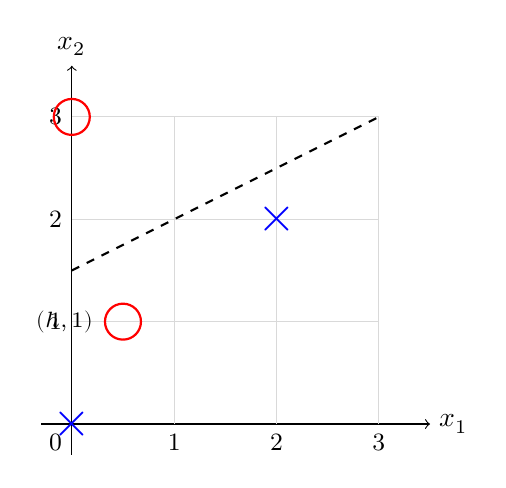
\begin{tikzpicture}[scale=1.3]
    % Axes
    \draw[->] (-0.3,0) -- (3.5,0) node[right] {$x_1$};
    \draw[->] (0,-0.3) -- (0,3.5) node[above] {$x_2$};
    
    % Grid lines (light gray)
    \foreach \x in {1,2,3} {
        \draw[gray!30, thin] (\x,0) -- (\x,3);
        \draw[gray!30, thin] (0,\x) -- (3,\x);
    }
    
    % Axis tick labels
    \foreach \x in {1,2,3} {
        \node[below, font=\small] at (\x,0) {\x};
        \node[left, font=\small] at (0,\x) {\x};
    }
    \node[below left, font=\small] at (0,0) {0};
    
    % Points (CORRECTED per user):
    % Circles (-1): at (0,3) and (h,1)
    \draw[red, thick] (0,3) circle (5pt);
    \draw[red, thick] (0.5,1) circle (5pt);
    \node[left, font=\footnotesize] at (0.3,1) {$(h,1)$};
    
    % Crosses (+1): at (0,0) and (2,2)
    \node[blue, scale=1.8] at (0,0) {$\times$};
    \node[blue, scale=1.8] at (2,2) {$\times$};
    
    % Decision boundary (dashed diagonal line)
    \draw[dashed, thick] (0,1.5) -- (3,3);
\end{tikzpicture}
\end{center}

\begin{question}[Θέμα 1.1]
\textbf{Πόσο μεγάλο μπορεί να είναι το $h$ ώστε οι δύο κλάσεις να είναι γραμμικώς διαχωρίσιμες; (0.5 μονάδες)}
\end{question}
\begin{answer}
\textit{(Πηγή: Lecture 6, slides 49--55)}

\textbf{Απάντηση:} $h_{max} = 1$.

\textbf{Εξήγηση:}
Τα σημεία της κλάσης +1 είναι τα $(0,0)$ και $(2,2)$, τα οποία ορίζουν το ευθύγραμμο τμήμα πάνω στην ευθεία $y=x$.
Τα σημεία της κλάσης -1 είναι τα $(0,3)$ και $(h,1)$.
Για να είναι οι κλάσεις διαχωρίσιμες, το σημείο $(h,1)$ δεν πρέπει να περάσει "κάτω" ή πάνω στο τμήμα των +1.
Επειδή το $(h,1)$ έχει $y=1$, αντικαθιστώντας στην ευθεία $y=x$ έχουμε $1=x \Rightarrow h=1$.
Αν $h=1$, το σημείο είναι το $(1,1)$, το οποίο βρίσκεται ακριβώς πάνω στο ευθύγραμμο τμήμα της κλάσης +1 (ανάμεσα στο 0,0 και 2,2).
Άρα, για $h < 1$ είναι διαχωρίσιμα. Οριακά, $h=1$.
\end{answer}

\begin{question}[Θέμα 1.2]
\textbf{Αλλάζει η κατεύθυνση του ορίου απόφασης μέγιστου περιθωρίου (maximum margin) συναρτήσει του $h$; (0.5 μονάδες)}
\end{question}
\begin{answer}
\textit{(Πηγή: Lecture 6, slides 49--55)}

\textbf{Όχι.}

\textbf{Εξήγηση:}
Το διάνυσμα βαρών $\mathbf{w}$ (που καθορίζει την κατεύθυνση) είναι κάθετο στο διαχωριστικό υπερεπίπεδο.
Για $h \in [0, 1)$, το εγγύτερο σημείο της κλάσης -1 προς την κλάση +1 είναι το $(h,1)$, και τα εγγύτερα της +1 βρίσκονται στο τμήμα $y=x$.
Λόγω της συμμετρίας των σημείων $(0,0)$ και $(2,2)$ ως προς το $(1,1)$, και της θέσης του $(h,1)$, η βέλτιστη διαχωριστική ευθεία διατηρεί σταθερή κλίση (παράλληλη με την $y=x$), απλά μετατοπίζεται (αλλάζει το bias) ή το πλάτος του margin στενεύει. Η διεύθυνση (κάθετη στην $y=x$) παραμένει αμετάβλητη (45 μοίρες), καθώς το "στενότερο" σημείο είναι πάντα μεταξύ της ευθείας $y=x$ και του σημείου $(h,1)$.
\end{answer}

\begin{question}[Θέμα 1.3]
\textbf{Ποια είναι η ελάχιστη και ποια η μέγιστη τιμή του πλάτους του περιθωρίου που επιτυγχάνεται με όριο απόφασης μέγιστου περιθωρίου για τα δεδομένα του σχήματος και γιατί; (1 μονάδα)}
\end{question}
\begin{answer}
\textit{(Πηγή: Lecture 6, slides 49--55)}

\textbf{Απάντηση:}
\begin{itemize}
    \item \textbf{Ελάχιστο Margin:} $0$ (όταν $h=1$)
    \item \textbf{Μέγιστο Margin:} $\frac{\sqrt{2}}{2} \approx 0.707$ (όταν $h=0$)
\end{itemize}

\textbf{Εξήγηση:}
Το margin καθορίζεται από την απόσταση του πλησιέστερου σημείου της κλάσης -1, δηλαδή του $P(h,1)$, από την ευθεία που διέρχεται από τα σημεία της κλάσης +1 (ευθεία $x - y = 0$).
Η απόσταση σημείου $(x_0, y_0)$ από ευθεία $Ax+By+C=0$ είναι $d = \frac{|Ax_0+By_0+C|}{\sqrt{A^2+B^2}}$.
Εδώ $A=1, B=-1, C=0$.
$$ d(h) = \frac{|1\cdot h - 1\cdot 1|}{\sqrt{1^2+(-1)^2}} = \frac{|h-1|}{\sqrt{2}} $$
\begin{itemize}
    \item Για $h=1: d = 0$. (Τα σημεία ταυτίζονται, μηδενικό margin).
    \item Για $h=0: d = \frac{|-1|}{\sqrt{2}} = \frac{1}{\sqrt{2}} = \frac{\sqrt{2}}{2}$.
\end{itemize}
\end{answer}

\subsection*{Θέμα 2 (SVM \& Ensembles)}

\begin{question}[Θέμα 2.1]
\textbf{Στο διπλανό σχήμα, ποια από τα σημεία εκπαίδευσης πρέπει να αφαιρέσουμε ώστε να αλλάξουν τα διανύσματα υποστήριξης; (1 μονάδα)}

\begin{center}
\begin{tikzpicture}[scale=0.8]
    \draw[->] (0,0) -- (6,0) node[right] {$x_1$};
    \draw[->] (0,0) -- (0,6) node[above] {$x_2$};
    
    % Decision boundary y = x
    \draw[dashed, thick] (0,0) -- (5.5,5.5);
    % Margin lines y = x + 1 and y = x - 1
    \draw[gray, dotted] (0,1) -- (4.5,5.5); % Upper margin
    \draw[gray, dotted] (1,0) -- (5.5,4.5); % Lower margin
    
    % Class 1: Crosses (Blue) - ABOVE the line
    % 3 Support Vectors on y = x + 1
    \node[blue] at (1,2) {$\times$};
    \node[blue] at (2,3) {$\times$};
    \node[blue] at (3,4) {$\times$};
    % Non-SVs
    \node[blue] at (1,4) {$\times$};
    \node[blue] at (2,5) {$\times$};
    \node[blue] at (0.5,3) {$\times$};
    \node[blue] at (1.5,5) {$\times$};
    \node[blue] at (0.5,4.5) {$\times$};
    \node[blue] at (2.5,4.5) {$\times$};
    
    % Class 2: Circles (Red) - BELOW the line
    % 3 Support Vectors on y = x - 1
    \node[red] at (2,1) {$\circ$};
    \node[red] at (3,2) {$\circ$};
    \node[red] at (4,3) {$\circ$};
    % Non-SVs
    \node[red] at (4,1) {$\circ$};
    \node[red] at (5,2) {$\circ$};
    \node[red] at (3,0.5) {$\circ$};
    \node[red] at (5,1) {$\circ$};
    \node[red] at (4.5,0.5) {$\circ$};
    \node[red] at (5.5,1.5) {$\circ$};
\end{tikzpicture}
\end{center}
\end{question}
\begin{answer}
\textit{(Πηγή: Lecture 6, slides 52--53)}
\textbf{Κανένα.} Η αφαίρεση μη-SVs δεν αλλάζει το margin.
\end{answer}

\begin{question}[Θέμα 2.2]
\textbf{Κάθε φορά που μεταβαίνω από γραμμικό SVM σε SVM με πολυωνυμικό kernel ανώτερης τάξης, περιμένω ότι τα διανύσματα υποστήριξης δεν θα αλλάξουν. Σωστό ή Λάθος; (2 μονάδες)}
\end{question}
\begin{answer}
\textit{(Πηγή: Lecture 6, slides 76--79)}
\textbf{Λάθος.} Τα SVs αλλάζουν ανάλογα με το kernel.
\end{answer}

\begin{question}[Θέμα 2.3]
\textbf{Στο διπλανό σχήμα φαίνεται η πρώτη απόφαση από τον αλγόριθμο AdaBoost για τέσσερα σημεία εκπαίδευσης. Τα βάρη που αποδίδονται στα τέσσερα σημεία εκπαίδευσης μετά από αυτή την απόφαση είναι $[\frac{1}{8}, \frac{1}{8}, \frac{1}{8}, \frac{5}{8}]$ (αντίστοιχη σειρά με το σχήμα). Σωστό ή Λάθος; (1 μονάδα)}

\begin{center}
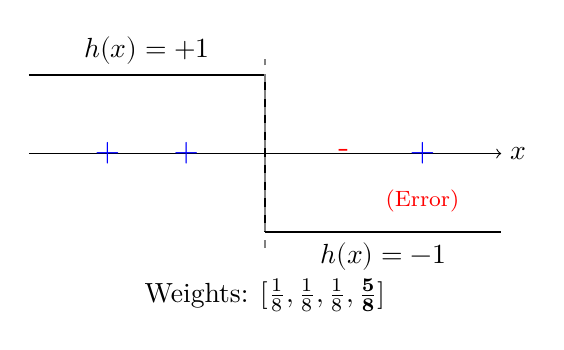
\begin{tikzpicture}[scale=1]
    % Axis / "Straight Line" where points lie
    \draw[->] (0,0) -- (6,0) node[right] {$x$};
    
    % Points on the axis (y=0)
    % Left Side (Predicted +1): Two +1 points
    \node[blue] at (1, 0) {\large +}; 
    \node[blue] at (2, 0) {\large +};
    
    % Right Side (Predicted -1): One -1 point, One +1 point (Error)
    \node[red] at (4, 0) {\large -};
    \node[blue] at (5, 0) {\large +}; % Misclassified
    
    % Decision Stump / "Pulse"
    % Level +1 above, Level -1 below
    \draw[thick] (0,1) -- (3,1) node[midway, above] {$h(x)=+1$}; % Top of pulse
    \draw[thick] (3,1) -- (3,-1); % Vertical transition
    \draw[thick] (3,-1) -- (6,-1) node[midway, below] {$h(x)=-1$}; % Bottom of pulse
    
    % Threshold line (optional, implicit in the vertical drop)
    \draw[dashed, gray] (3,-1.2) -- (3,1.2);
    
    % Error indication
    \node[red, font=\footnotesize] at (5, -0.6) {(Error)};
    
    % Weights indication
    \node at (3, -1.8) {Weights: $[\frac{1}{8}, \frac{1}{8}, \frac{1}{8}, \mathbf{\frac{5}{8}}]$};
\end{tikzpicture}
\end{center}
\end{question}

\begin{answer}
\textit{(Πηγή: Lecture 8, slides 31--34)}
\textbf{Σωστό.} (Υπόθεση: $\alpha_t \approx \ln((1-\epsilon)/\epsilon)$). Αν το σφάλμα είναι 1/4, το weight update αυξάνει το βάρος του λάθους και μειώνει των σωστών.
\end{answer}

\subsection*{Θέμα 3 (Logistic Regression)}

\begin{question}[Θέμα 3.1]
\textbf{Αν εκπαιδεύσουμε ένα logistic regression μοντέλο μεγιστοποιώντας την πιθανοφάνεια των ετικετών, δεδομένων των σημείων εκπαίδευσης, καταλήγουμε σε πολλαπλές τοπικά βέλτιστες λύσεις. Ναι ή όχι; (2 μονάδες)}
\end{question}
\begin{answer}
\textit{(Πηγή: Lecture 5, slides 78--80)}
\textbf{Όχι.} Η συνάρτηση κόστους (Negative Log Likelihood) για την Logistic Regression είναι \textbf{κυρτή} (convex), άρα έχει \textbf{μοναδικό ολικό ελάχιστο}.
\end{answer}

\begin{question}[Θέμα 3.2]
\textbf{Αν εκπαιδεύσουμε ένα logistic regression μοντέλο με Stochastic Gradient Descent (SGD) αλγόριθμο με σταθερό ρυθμό μάθησης, τότε θα καταλήξουμε στα ακριβή, βέλτιστα βάρη. Συμφωνείτε ή όχι και γιατί; (2 μονάδες)}
\end{question}
\begin{answer}
\textit{(Πηγή: Lecture 5)}
\textbf{Όχι.} Με σταθερό learning rate, ο SGD \textbf{ταλαντώνεται} γύρω από το ελάχιστο και δεν συγκλίνει ποτέ σε ένα σημείο (θόρυβος λόγω στοχαστικότητας). Για σύγκλιση απαιτείται μείωση του ρυθμού μάθησης (learning rate decay).
\end{answer}

\clearpage
\section{Φεβρουάριος 2025}

\textit{Εξεταστική Φεβρουαρίου - Φεβρουάριος 2025}

\subsection*{Θέμα 1 (Model Selection)}

\begin{question}[Θέμα 1.1]
\textbf{Α)} Για τα παρακάτω σχήματα Train vs Test error, χαρακτηρίστε ποιο μοντέλο κάνει underfitting, overfitting και καλή γενίκευση.

\begin{center}
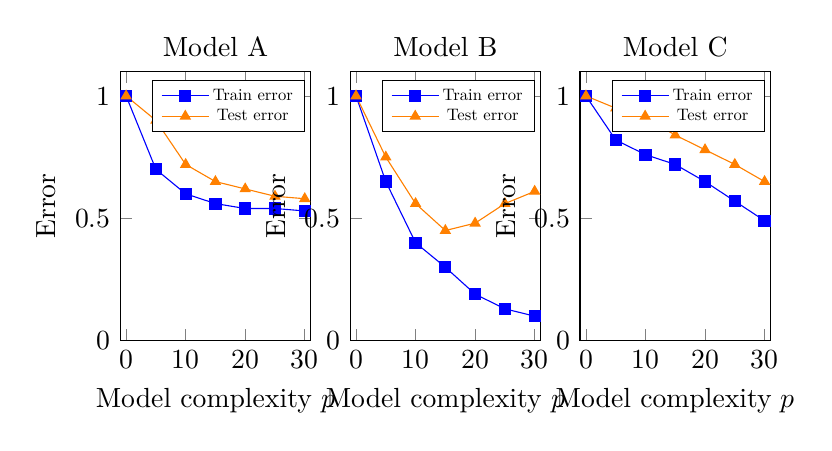
\begin{tikzpicture}
    % Model A
    \begin{axis}[
        name=plotA,
        width=0.33\linewidth, height=5cm,
        xmin=-1, xmax=31, ymin=0, ymax=1.1,
        title={Model A},
        xlabel={Model complexity $p$},
        ylabel={Error},
        legend pos=north east,
        legend style={nodes={scale=0.6, transform shape}},
        title style={yshift=-1ex}
    ]
        \addplot[blue, mark=cube*] coordinates {(0,1) (5,0.7) (10,0.6) (15,0.56) (20,0.54) (25,0.54) (30,0.53)};
        \addlegendentry{Train error}
        \addplot[orange, mark=triangle*] coordinates {(0,1) (5,0.9) (10,0.72) (15,0.65) (20,0.62) (25,0.59) (30,0.58)};
        \addlegendentry{Test error}
    \end{axis}

    % Model B
    \begin{axis}[
        name=plotB,
        at={($(plotA.east)+(0.5cm,0)$)},
        anchor=west,
        width=0.33\linewidth, height=5cm,
        xmin=-1, xmax=31, ymin=0, ymax=1.1,
        title={Model B},
        xlabel={Model complexity $p$},
        ylabel={Error},
        legend pos=north east,
        legend style={nodes={scale=0.6, transform shape}},
        title style={yshift=-1ex}
    ]
        \addplot[blue, mark=cube*] coordinates {(0,1) (5,0.65) (10,0.4) (15,0.3) (20,0.19) (25,0.13) (30,0.1)};
        \addlegendentry{Train error}
        \addplot[orange, mark=triangle*] coordinates {(0,1) (5,0.75) (10,0.56) (15,0.45) (20,0.48) (25,0.56) (30,0.61)};
        \addlegendentry{Test error}
    \end{axis}

    % Model C
    \begin{axis}[
        name=plotC,
        at={($(plotB.east)+(0.5cm,0)$)},
        anchor=west,
        width=0.33\linewidth, height=5cm,
        xmin=-1, xmax=31, ymin=0, ymax=1.1,
        title={Model C},
        xlabel={Model complexity $p$},
        ylabel={Error},
        legend pos=north east,
        legend style={nodes={scale=0.6, transform shape}},
        title style={yshift=-1ex}
    ]
        \addplot[blue, mark=cube*] coordinates {(0,1) (5,0.82) (10,0.76) (15,0.72) (20,0.65) (25,0.57) (30,0.49)};
        \addlegendentry{Train error}
        \addplot[orange, mark=triangle*] coordinates {(0,1) (5,0.95) (10,0.91) (15,0.84) (20,0.78) (25,0.72) (30,0.65)};
        \addlegendentry{Test error}
    \end{axis}
\end{tikzpicture}
\end{center}
\end{question}

\begin{answer}
\textit{(Πηγή: Lecture 1, slides 35--38)}

\begin{itemize}
    \item \textbf{Model A: Underfitting.} Οι τιμές σφάλματος (train και test) παραμένουν υψηλές και κοντά μεταξύ τους, υποδεικνύοντας ότι το μοντέλο είναι πολύ απλό για να μάθει τα δεδομένα.
    \item \textbf{Model B: Overfitting.} Το σφάλμα εκπαίδευσης (train) γίνεται πολύ μικρό, αλλά το σφάλμα ελέγχου (test) αρχίζει να αυξάνεται μετά από ένα σημείο ($\rho = 15$), δημιουργώντας μεγάλο χάσμα.
    \item \textbf{Model C: Καλή γενίκευση.} Τα σφάλματα μειώνονται σταθερά και παραμένουν κοντά, χωρίς το μοντέλο να "απομνημονεύει" τα δεδομένα εκπαίδευσης όπως το Model B.
\end{itemize}
\end{answer}

\begin{question}[Θέμα 1.2]
\textbf{Β)} Κάποιος ισχυρίζεται ότι αυξάνοντας την παράμετρο $C$ στον soft margin SVM ταξινομητή θα αυξηθεί και το περιθώριο ταξινόμησης (margin). Συμφωνείτε μαζί του;
\end{question}

\begin{answer}
\textit{(Πηγή: Lecture 6, slides 60--65)}
\textbf{Απ: Λάθος.} Μεγαλύτερο $C$ σημαίνει μεγαλύτερη ποινή για σφάλματα, άρα \textbf{μικρότερο margin} (πιο σκληρό όριο).
\end{answer}

\begin{question}[Θέμα 1.3]
\textbf{Γ)} Σε ένα soft margin SVM ταξινομητή οι βοηθητικές μεταβλητές $\xi_i$ που συνοδεύουν κάθε ένα από τα δείγματα $x_i$, έχουν μη μηδενική τιμή για (μπορεί παραπάνω από ένα να είναι σωστά):
\begin{enumerate}
    \item[α)] λάθος ταξινομημένα (misclassified) $x_i$
    \item[β)] σωστά ταξινομημένα $x_i$
    \item[γ)] $x_i$ τα οποία είναι εντός του περιθωρίου (margin)
    \item[δ)] $x_i$ τα οποία είναι εκτός του περιθωρίου (margin)
\end{enumerate}
Αιτιολογήστε την απάντησή σας.
\end{question}

\begin{answer}
\textbf{Απ: α, γ.} Οι slack variables $\xi_i > 0$ όταν το σημείο είναι:
\begin{itemize}
    \item Λάθος ταξινομημένο ($\xi_i > 1$)
    \item Εντός του margin αλλά σωστά ταξινομημένο ($0 < \xi_i \leq 1$)
\end{itemize}
\textit{(Πηγή: Lecture 6, slides 60--65)}
\end{answer}

\begin{question}[Θέμα 1.4]
\textbf{Δ)} Για ένα νευρωνικό δίκτυο ταξινόμησης με δύο εισόδους (2 features), 20 νευρώνες στο hidden layer και 10 νευρώνες στο output layer:
\begin{enumerate}
    \item[α)] Χρησιμοποιούμε softmax για το output layer. \textbf{Σωστό/Λάθος;}
    \item[β)] Είναι σωστό να χρησιμοποιούμε γραμμική activation στο hidden layer. \textbf{Σωστό/Λάθος;}
    \item[γ)] Το δίκτυο έχει 240 παραμέτρους. \textbf{Σωστό/Λάθος;}
\end{enumerate}
\end{question}

\begin{answer}
\textit{(Πηγή: Lecture 7, slides 1--2, 28--30)}
\begin{itemize}
    \item \textbf{α) Σωστό.} Για multi-class classification χρησιμοποιούμε softmax.
    \item \textbf{β) Λάθος.} Γραμμική activation στο hidden layer καταργεί τη δυνατότητα μη-γραμμικού διαχωρισμού.
    \item \textbf{γ) Λάθος.} Υπολογισμός:
    \begin{itemize}
        \item Hidden layer: $(2+1) \times 20 = 60$ παράμετροι
        \item Output layer: $(20+1) \times 10 = 210$ παράμετροι
        \item \textbf{Σύνολο: $60 + 210 = 270$ παράμετροι}
    \end{itemize}
\end{itemize}
\end{answer}

\subsection*{Θέμα 2 (SVM Exercise)}

\begin{question}[Θέμα 2.1]
Στο διπλανό σχήμα φαίνονται τα δεδομένα εκπαίδευσης για ένα πρόβλημα δυαδικής ταξινόμησης (binary classification problem).
Βρείτε το όριο απόφασης $w^T x + w_0 = 0$ που μεγιστοποιεί το περιθώριο μεταξύ των κλάσεων (maximum margin) με βάση τη θεωρία των SVM ταξινομητών και τις παραδοχές που τη συνοδεύουν. Ποια είναι τα διανύσματα υποστήριξης και πόσο είναι το μέγιστο περιθώριο;

\begin{center}
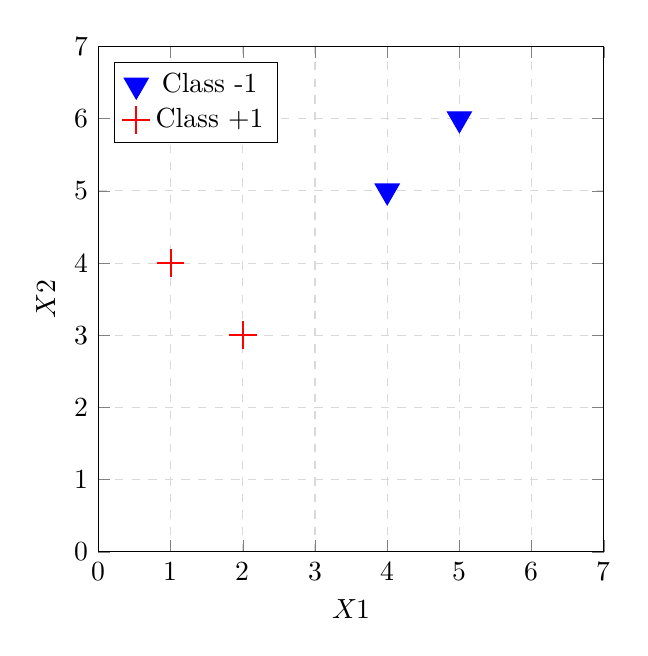
\begin{tikzpicture}
    \begin{axis}[
        width=8cm, height=8cm,
        xmin=0, xmax=7, ymin=0, ymax=7,
        xlabel={$X1$}, ylabel={$X2$},
        grid=both,
        grid style={dashed, gray!30},
        xtick={0,1,2,3,4,5,6,7},
        ytick={0,1,2,3,4,5,6,7},
        legend pos=north west,
        clip=false
    ]
        \addplot[only marks, blue, mark=triangle*, mark size=5pt, mark options={rotate=180}] coordinates {(4,5) (5,6)};
        \addlegendentry{Class -1}
        \addplot[only marks, red, mark=+, mark size=5pt, thick] coordinates {(1,4) (2,3)};
        \addlegendentry{Class +1}
    \end{axis}
\end{tikzpicture}
\end{center}
\end{question}

\begin{answer}
\textbf{Λύση:}

\textbf{1. Αναγνώριση Δεδομένων:}
Από το σχήμα έχουμε δύο κλάσεις:
\begin{itemize}
    \item \textbf{Class +1 (Red crosses):} $x^{(1)}=(1,4), x^{(2)}=(2,3)$
    \item \textbf{Class -1 (Blue triangles):} $x^{(3)}=(4,5), x^{(4)}=(5,6)$
\end{itemize}

\textbf{2. Εύρεση Διαχωριστικής Ευθείας:}
Παρατηρούμε ότι τα δεδομένα διαχωρίζονται γραμμικά. Η βέλτιστη ευθεία (maximum margin) θα βρίσκεται ακριβώς στη μέση της απόστασης των πλησιέστερων σημείων των δύο κλάσεων.
Τα πλησιέστερα σημεία είναι τα $x^{(1)}, x^{(2)}$ από την Class +1 και το $x^{(3)}$ από την Class -1.
Αυτά σχηματίζουν τα **Support Vectors**.

Η κατεύθυνση διαχωρισμού είναι διαγώνια. Παρατηρούμε ότι για τα +1 ισχύει $x_1+x_2 = 5$ (σημεία (1,4) και (2,3)).
Για το πλησιέστερο -1 ισχύει $x_1+x_2 = 9$ (σημείο (4,5)).

Η διαχωριστική ευθεία θα είναι η μεσοκάθετος, άρα θα έχει εξίσωση της μορφής $x_1 + x_2 = C$.
Το $C$ είναι ο μέσος όρος των αθροισμάτων: $C = \frac{5+9}{2} = 7$.

Άρα η εξίσωση του ορίου απόφασης είναι:
$$ x_1 + x_2 - 7 = 0 $$

Για να την φέρουμε στην κανονική μορφή SVM ($w^T x + w_0 = 0$), όπου $y_i(w^T x_i + w_0) \ge 1$ για τα Support Vectors, ελέγχουμε:
Για Class +1 ($y=1$): θέλουμε $w^T x + w_0 \ge 1$.
Για Class -1 ($y=-1$): θέλουμε $w^T x + w_0 \le -1$.

Η εξίσωση $-(x_1 + x_2 - 7) = 0 \Rightarrow -x_1 - x_2 + 7 = 0$ δίνει:
Για $x^{(1)}$ (sum=5): $-5+7 = 2$.
Για $x^{(3)}$ (sum=9): $-9+7 = -2$.
Για να έχουμε περιθώριο 1, διαιρούμε με το 2:
$$ -0.5 x_1 - 0.5 x_2 + 3.5 = 0 $$
Άρα $\mathbf{w} = [-0.5, -0.5]^T$ και $w_0 = 3.5$.

\textbf{3. Υπολογισμός Περιθωρίου (Margin):}
Το margin $M$ δίνεται από τον τύπο $M = \frac{2}{||w||}$.
$$ ||w|| = \sqrt{(-0.5)^2 + (-0.5)^2} = \sqrt{0.25 + 0.25} = \sqrt{0.5} = \frac{1}{\sqrt{2}} $$
$$ M = \frac{2}{1/\sqrt{2}} = 2\sqrt{2} \approx \mathbf{2.828} $$

\textbf{Απαντήσεις:}
\begin{itemize}
    \item \textbf{Όριο απόφασης:} $-0.5 x_1 - 0.5 x_2 + 3.5 = 0$ (ή ισοδύναμα $x_1 + x_2 - 7 = 0$)
    \item \textbf{Support Vectors:} $(1,4), (2,3)$ από Class +1 και $(4,5)$ από Class -1.
    \item \textbf{Μέγιστο Περιθώριο:} $2\sqrt{2}$.
\end{itemize}

\begin{center}
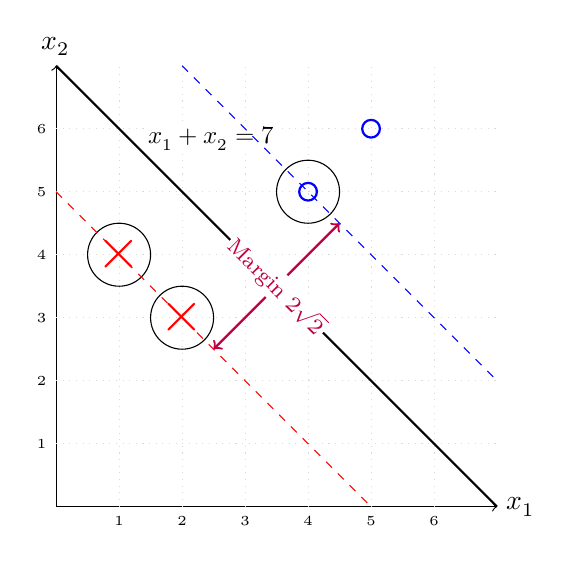
\begin{tikzpicture}[scale=0.8]
    \draw[->] (0,0) -- (7,0) node[right] {$x_1$};
    \draw[->] (0,0) -- (0,7) node[above] {$x_2$};
    \foreach \x in {1,2,3,4,5,6} {
        \draw[gray!30, thin, dotted] (\x,0) -- (\x,7);
        \draw[gray!30, thin, dotted] (0,\x) -- (7,\x);
        \node[below, font=\tiny] at (\x,0) {\x};
        \node[left, font=\tiny] at (0,\x) {\x};
    }
    
    % Class +1 (Red Crosses)
    \node[red, font=\huge] at (1,4) {$\mathbf{\times}$};
    \node[red, font=\huge] at (2,3) {$\mathbf{\times}$};
    % Class -1 (Blue Circles)
    \draw[blue, thick] (4,5) circle (4pt);
    \draw[blue, thick] (5,6) circle (4pt);
    
    % Support Vectors (Highlight)
    \draw[black, thin] (1,4) circle (0.5);
    \draw[black, thin] (2,3) circle (0.5);
    \draw[black, thin] (4,5) circle (0.5);
    
    % Decision Boundary: x1 + x2 = 7
    \draw[thick, black] (0,7) -- (7,0) node[pos=0.2, above right, fill=white, inner sep=1pt] {\small $x_1+x_2=7$};
    
    % Margins
    % +1 Margin: x1 + x2 = 5
    \draw[dashed, red] (0,5) -- (5,0);
    % -1 Margin: x1 + x2 = 9
    \draw[dashed, blue] (2,7) -- (7,2);
    
    % Margin Width Arrow
    \draw[<->, purple, thick] (2.5, 2.5) -- (4.5, 4.5) node[midway, fill=white, inner sep=1pt, rotate=-45] {\footnotesize Margin $2\sqrt{2}$};
\end{tikzpicture}
\end{center}
\end{answer}

\subsection*{Θέμα 3 (Kernel \& PCA)}

\begin{question}[Θέμα 3.1]
\textbf{Α)} Σε τι διάσταση (αριθμό) προβάλει έμμεσα τα διανύσματα $x \in \mathbb{R}^2$, η συνάρτηση, $K(x, z) = (1 + x^T z)^2$; Αιτιολογήστε την απάντησή σας.
\end{question}

\begin{answer}
\textit{(Πηγή: Lecture 6, slide 76)}

\textbf{Ανάλυση:}
Αναπτύσσουμε το πολυωνυμικό kernel για $x = (x_1, x_2)$ και $z = (z_1, z_2)$:
$$ K(x, z) = (1 + x_1 z_1 + x_2 z_2)^2 = (1 + x_1 z_1 + x_2 z_2)(1 + x_1 z_1 + x_2 z_2) $$
$$ = 1 + x_1 z_1 + x_2 z_2 + x_1 z_1 + x_1^2 z_1^2 + x_1 x_2 z_1 z_2 + x_2 z_2 + x_1 x_2 z_1 z_2 + x_2^2 z_2^2 $$
$$ = 1 + 2x_1 z_1 + 2x_2 z_2 + 2x_1 x_2 z_1 z_2 + x_1^2 z_1^2 + x_2^2 z_2^2 $$

Αυτό μπορεί να γραφτεί ως εσωτερικό γινόμενο $\Phi(x)^T \Phi(z)$ με:
$$ \Phi(x) = [1, \sqrt{2}x_1, \sqrt{2}x_2, \sqrt{2}x_1 x_2, x_1^2, x_2^2]^T $$

\textbf{Απάντηση:}
Η διάσταση του feature space είναι \textbf{6}.
\end{answer}

\begin{question}[Θέμα 3.2]
\textbf{Β)} Ποια (-ες) από τις παρακάτω δύο προτάσεις είναι σωστή (-ές) και ποια (-ες) λάθος σχετικά με την Ανάλυση Πρωτευουσών Συνιστωσών (Principal Component Analysis) και γιατί;
\begin{enumerate}
    \item[α)] Προσθέτοντας μονάδα (1) στο τέλος κάθε διανύσματος δεν αλλάζει ουσιαστικά το αποτέλεσμα του PCA.
    \item[β)] Αν χρησιμοποιήσω τη μέθοδο PCA για να προβάλω διανύσματα $d$ διάστασης σε $j$ πρωτεύουσες συνιστώσες (principal components) και κατόπιν για να προβάλω τα διανύσματα $j$ διάστασης (μετά την πρώτη προβολή) σε $k$ πρωτεύουσες συνιστώσες όπου $d > j > k$, θα πάρω το ίδιο αποτέλεσμα με το εάν χρησιμοποιήσω τη μέθοδο PCA για να προβάλω τα διανύσματα $d$ διάστασης κατευθείαν σε $k$ πρωτεύουσες συνιστώσες.
\end{enumerate}
\end{question}

\begin{answer}
\textit{(Πηγή: Lecture 9-10, slides 52--54)}

\begin{itemize}
    \item \textbf{α) Σωστή.} Η προσθήκη μιας σταθερής τιμής (όπως το 1) σε κάθε δείγμα δεν επηρεάζει τον πίνακα συνδιακύμανσης (covariance matrix), καθώς η διακύμανση (variance) μιας σταθεράς είναι μηδέν. Επομένως, τα ιδιοδιανύσματα και οι ιδιοτιμές παραμένουν αναλλοίωτα.
    \item \textbf{β) Σωστή.} Το PCA βρίσκει τις κατευθύνσεις μέγιστης διακύμανσης. Οι $k$ πρώτες συνιστώσες ενός συνόλου δεδομένων είναι οι ίδιες είτε τις εξάγουμε απευθείας, είτε περνώντας από έναν ενδιάμεσο χώρο $j$ διαστάσεων ($j > k$), καθώς τα principal components είναι ορθογώνια μεταξύ τους και διατεταγμένα κατά φθίνουσα διακύμανση.
\end{itemize}
\end{answer}

\subsection*{Θέμα 4 (1D Classification)}

\begin{question}[Θέμα 4.1]
Θεωρήστε το μονοδιάστατο πρόβλημα ταξινόμησης του παρακάτω σχήματος. Ποιο επιπλέον χαρακτηριστικό θα προσθέτατε στο $x$ ώστε να κάνετε τα δείγματα γραμμικά διαχωρίσιμα στο νέο δισδιάστατο χώρο; Εκφράστε το συναρτήσει του $x$.

\begin{center}
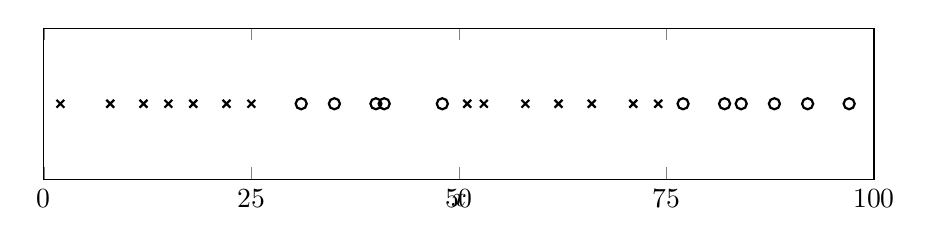
\begin{tikzpicture}
    \begin{axis}[
        width=1.0\linewidth,
        height=3.5cm,
        axis lines=box,
        xmin=0, xmax=100,
        ymin=-0.5, ymax=0.5,
        xtick={0, 25, 50, 75, 100},
        ytick=\empty,
        xlabel={$x$},
        xlabel style={at={(ticklabel* cs:0.5)},anchor=north, yshift=-2pt},
        clip=false
    ]
        % Class x
        \addplot[only marks, mark=x, thick] coordinates {
            (2,0) (8,0) (12,0) (15,0) (18,0) (22,0) (25,0)
            (51,0) (53,0) (58,0) (62,0) (66,0) (71,0) (74,0)
        };
        % Class o
        \addplot[only marks, mark=o, thick] coordinates {
            (31,0) (35,0) (40,0) (41,0) (48,0)
            (77,0) (82,0) (84,0) (88,0) (92,0) (97,0)
        };
    \end{axis}
\end{tikzpicture}
\end{center}
\end{question}

\begin{answer}
\textit{(Πηγή: Lecture 6, slides 76--78)}

\textbf{Ανάλυση:}
Παρατηρώντας το σχήμα, τα δεδομένα ανήκουν σε δύο κλάσεις ($x$ και $o$) που εναλλάσσονται σε διαστήματα κατά μήκος του άξονα $x$. Συγκεκριμένα:
\begin{itemize}
    \item Κλάση 1 ($x$): $[0, 25]$ και $[50, 75]$
    \item Κλάση 2 ($o$): $[25, 50]$ και $[75, 100]$
\end{itemize}

Στον μονοδιάστατο χώρο τα δεδομένα δεν είναι γραμμικά διαχωρίσιμα. Για να γίνουν διαχωρίσιμα σε 2D, πρέπει να προσθέσουμε ένα χαρακτηριστικό $y = f(x)$ τέτοιο ώστε η διαχωριστική ευθεία $w_1 x + w_2 y + w_0 = 0$ να μπορεί να τα χωρίσει.

\textbf{Προτεινόμενη Λύση:}
Χρειαζόμαστε μια συνάρτηση που να αλλάζει πρόσημο στα σημεία "επαφής" των κλάσεων (25, 50, 75). Μια απλή επιλογή είναι ένα πολυώνυμο 3ου βαθμού:
$$ f(x) = (x - 25)(x - 50)(x - 75) $$

Αυτή η συνάρτηση:
\begin{itemize}
    \item Είναι θετική για $x \in (25, 50)$ και $x > 75$.
    \item Είναι αρνητική για $x < 25$ και $x \in (50, 75)$.
\end{itemize}
Έτσι, τα δείγματα της μίας κλάσης θα έχουν θετικές τιμές στο νέο χαρακτηριστικό και της άλλης αρνητικές (σε συγκεκριμένα διαστήματα), επιτρέποντας έναν γραμμικό διαχωρισμό.

\textbf{Εναλλακτική Λύση:}
Μια περιοδική συνάρτηση όπως η $\sin$ ή η $\cos$ (με κατάλληλη περίοδο):
$$ f(x) = \sin\left(\frac{2\pi x}{50}\right) $$
Η συνάρτηση αυτή αλλάζει πρόσημο κάθε 25 μονάδες, "σηκώνοντας" τα δείγματα της μίας κλάσης πάνω από τον άξονα $x$ και της άλλης κάτω από αυτόν.

\textbf{Απάντηση:}
Το επιπλέον χαρακτηριστικό μπορεί να είναι η συνάρτηση $y = (x - 25)(x - 50)(x - 75)$ ή $y = \sin\left(\frac{2\pi x}{50}\right)$.
\end{answer}

\clearpage
\section{Ερωτήσεις Εξάσκησης}

\textit{Επιπλέον ερωτήσεις για εξάσκηση που καλύπτουν όλη την ύλη του μαθήματος.}


\begin{question}[Θέμα 1]
\textbf{Σε ένα ιατρικό test, η ευαισθησία (sensitivity) είναι 95\% και η ειδικότητα (specificity) είναι 90\%. Αν η επικράτηση (prevalence) της νόσου είναι 1\%, ποια είναι η πιθανότητα κάποιος να είναι πράγματι άρρωστος δεδομένου θετικού test;}
\end{question}

\begin{answer}
\textit{(Πηγή: Lecture 3, slides 22--24)}

Δεδομένα:
\begin{itemize}
    \item $P(\text{Test+}|\text{Νόσος}) = 0.95$ (sensitivity)
    \item $P(\text{Test-}|\text{Υγιής}) = 0.90 \Rightarrow P(\text{Test+}|\text{Υγιής}) = 0.10$ (false positive)
    \item $P(\text{Νόσος}) = 0.01$
\end{itemize}

Εφαρμόζουμε Bayes:
$$ P(\text{Νόσος}|\text{Test+}) = \frac{P(\text{Test+}|\text{Νόσος}) \cdot P(\text{Νόσος})}{P(\text{Test+})} $$

Όπου:
$$ P(\text{Test+}) = 0.95 \cdot 0.01 + 0.10 \cdot 0.99 = 0.0095 + 0.099 = 0.1085 $$

$$ P(\text{Νόσος}|\text{Test+}) = \frac{0.95 \cdot 0.01}{0.1085} = \frac{0.0095}{0.1085} \approx \mathbf{8.76\%} $$

\textbf{Συμπέρασμα:} Παρά το υψηλό sensitivity, η χαμηλή prevalence οδηγεί σε πολλά false positives.
\end{answer}

\begin{question}[Θέμα 2]
\textbf{Εξηγήστε γιατί ο αλγόριθμος k-NN αποτυγχάνει σε υψηλές διαστάσεις (curse of dimensionality) και προτείνετε τρόπους αντιμετώπισης.}
\end{question}

\begin{answer}
\textit{(Πηγή: Lecture 2, slides 67--72)}

\textbf{Πρόβλημα:}
\begin{itemize}
    \item Σε υψηλές διαστάσεις, όλα τα σημεία απέχουν \textbf{σχεδόν ίση απόσταση} μεταξύ τους.
    \item Η έννοια του "γείτονα" χάνει νόημα.
    \item Ο όγκος του χώρου αυξάνεται εκθετικά, άρα χρειάζονται εκθετικά περισσότερα δεδομένα.
\end{itemize}

\textbf{Αντιμετώπιση:}
\begin{enumerate}
    \item \textbf{Μείωση διαστάσεων:} PCA, LDA, t-SNE
    \item \textbf{Feature selection:} Επιλογή σχετικών χαρακτηριστικών
    \item \textbf{Weighted distance:} Χρήση βαρών σε κάθε διάσταση
    \item \textbf{Locality-Sensitive Hashing:} Για approximate nearest neighbors
\end{enumerate}
\end{answer}

\begin{question}[Θέμα 3]
\textbf{Δεδομένα: 10 δείγματα, 6 θετικά (+) και 4 αρνητικά (-). Μετά από split σε χαρακτηριστικό $X$:
\begin{itemize}
    \item Αριστερός κόμβος: 4+, 1-
    \item Δεξιός κόμβος: 2+, 3-
\end{itemize}
Υπολογίστε το Information Gain.}
\end{question}

\begin{answer}
\textit{(Πηγή: Lecture 8, slides 68--72)}

\textbf{Entropy πριν το split:}
$$ H(S) = -\frac{6}{10}\log_2\frac{6}{10} - \frac{4}{10}\log_2\frac{4}{10} = 0.971 \text{ bits} $$

\textbf{Entropy μετά το split:}
\begin{itemize}
    \item Αριστερός: $H(L) = -\frac{4}{5}\log_2\frac{4}{5} - \frac{1}{5}\log_2\frac{1}{5} = 0.722$
    \item Δεξιός: $H(R) = -\frac{2}{5}\log_2\frac{2}{5} - \frac{3}{5}\log_2\frac{3}{5} = 0.971$
\end{itemize}

$$ H(S|X) = \frac{5}{10} \cdot 0.722 + \frac{5}{10} \cdot 0.971 = 0.847 $$

\textbf{Information Gain:}
$$ IG(S, X) = H(S) - H(S|X) = 0.971 - 0.847 = \mathbf{0.124 \text{ bits}} $$
\end{answer}

\begin{question}[Θέμα 4]
\textbf{Ο αλγόριθμος Perceptron εγγυάται σύγκλιση αν τα δεδομένα είναι γραμμικά διαχωρίσιμα. Αν δεν είναι, τι συμβαίνει; Πώς το αντιμετωπίζουμε;}
\end{question}

\begin{answer}
\textit{(Πηγή: Lecture 5, slides 26--31)}

\textbf{Αν τα δεδομένα ΔΕΝ είναι γραμμικά διαχωρίσιμα:}
\begin{itemize}
    \item Ο Perceptron \textbf{δεν συγκλίνει} --- ταλαντώνεται επ' αόριστον.
    \item Τα βάρη αλλάζουν συνεχώς χωρίς να φτάσουν σε σταθερή λύση.
\end{itemize}

\textbf{Λύσεις:}
\begin{itemize}
    \item \textbf{Pocket Algorithm:} Κρατάμε τα καλύτερα βάρη που βρέθηκαν μέχρι στιγμής (με το μικρότερο training error).
    \item \textbf{Soft-margin SVM:} Επιτρέπουμε κάποια σφάλματα με ποινή (C).
    \item \textbf{Kernel trick:} Μετασχηματισμός σε υψηλότερη διάσταση όπου μπορεί να είναι γραμμικά διαχωρίσιμα.
    \item \textbf{Multi-layer Perceptron:} Χρήση νευρωνικού δικτύου για μη-γραμμικά όρια.
\end{itemize}
\end{answer}

\begin{question}[Θέμα 5]
\textbf{Συγκρίνετε τη μέθοδο Hold-out validation με την k-Fold Cross-Validation. Πότε προτιμάμε την κάθε μία;}
\end{question}

\begin{answer}
\textit{(Πηγή: Lecture 2, slides 54--58)}

\begin{center}
\begin{tabular}{|l|c|c|}
\hline
\textbf{Κριτήριο} & \textbf{Hold-out} & \textbf{k-Fold CV} \\
\hline
Χρόνος & Γρήγορο & k φορές πιο αργό \\
Variance εκτίμησης & Υψηλό & Χαμηλό \\
Bias εκτίμησης & Υψηλό (αν μικρό set) & Χαμηλό \\
Αξιοποίηση δεδομένων & 70-80\% & 100\% \\
\hline
\end{tabular}
\end{center}

\begin{itemize}
    \item \textbf{Προτιμάμε Hold-out:} Μεγάλα datasets, ακριβά μοντέλα (π.χ. deep learning).
    \item \textbf{Προτιμάμε k-Fold CV:} Μικρά datasets, όταν χρειάζεται σταθερή/αξιόπιστη εκτίμηση.
\end{itemize}
\end{answer}

\begin{question}[Θέμα 6]
\textbf{Εξηγήστε τη διαφορά μεταξύ L1 (Lasso) και L2 (Ridge) regularization. Πότε χρησιμοποιούμε το καθένα;}
\end{question}

\begin{answer}
\textit{(Πηγή: Lecture 5, slides 68--72)}

\textbf{L2 Regularization (Ridge):} $J = \text{Loss} + \lambda \sum w_i^2$
\begin{itemize}
    \item Μειώνει τα βάρη αλλά \textbf{δεν τα μηδενίζει} (smooth solution).
    \item Χρήση: Όταν όλα τα features είναι σημαντικά.
\end{itemize}

\textbf{L1 Regularization (Lasso):} $J = \text{Loss} + \lambda \sum |w_i|$
\begin{itemize}
    \item \textbf{Μηδενίζει} κάποια βάρη $\rightarrow$ \textbf{feature selection} (sparse solution).
    \item Χρήση: Όταν θέλουμε επιλογή χαρακτηριστικών ή interpretability.
\end{itemize}
\end{answer}

\begin{question}[Θέμα 7]
\textbf{Συγκρίνετε Batch Gradient Descent, Stochastic Gradient Descent (SGD) και Mini-batch GD.}
\end{question}

\begin{answer}
\textit{(Πηγή: Lecture 7, slides 59--61)}

\begin{center}
\begin{tabular}{|l|c|c|c|}
\hline
& \textbf{Batch GD} & \textbf{SGD} & \textbf{Mini-batch} \\
\hline
Samples/update & Όλα (N) & 1 & b (π.χ. 32-256) \\
Noise gradient & Καθόλου & Πολύ & Μέτριο \\
Σύγκλιση & Σταθερή & Ταλάντωση & Καλή ισορροπία \\
Χρόνος/epoch & Αργό & Γρήγορο & Μέτριο \\
\hline
\end{tabular}
\end{center}

\textbf{Συμπέρασμα:} Mini-batch GD είναι η πιο συνήθης επιλογή (π.χ. με Adam).
\end{answer}

\begin{question}[Θέμα 8]
\textbf{Αναφέρετε τρεις περιορισμούς του k-Means και προτείνετε εναλλακτικές.}
\end{question}

\begin{answer}
\textit{(Πηγή: Lecture 9-10, slides 5--10)}

\textbf{Περιορισμοί:}
\begin{itemize}
    \item Πρέπει να γνωρίζουμε το $k$ εκ των προτέρων.
    \item Υποθέτει σφαιρικά clusters (αποτυγχάνει σε πολύπλοκα σχήματα).
    \item Ευαισθησία στην αρχικοποίηση (τοπικά ελάχιστα).
    \item Ευαισθησία σε outliers.
\end{itemize}

\textbf{Εναλλακτικές:}
\begin{itemize}
    \item \textbf{k-Means++:} Καλύτερη αρχικοποίηση.
    \item \textbf{GMM:} Για ελλειπτικά clusters (soft assignment).
    \item \textbf{DBSCAN:} Αυτόματο $k$, ανθεκτικό σε θόρυβο και τυχαία σχήματα.
    \item \textbf{Spectral Clustering:} Για μη-κυρτά clusters.
\end{itemize}
\end{answer}

\begin{question}[Θέμα 9]
\textbf{Ποιες είναι οι βασικές διαφορές μεταξύ k-Means και Gaussian Mixture Models (GMM);}
\end{question}

\begin{answer}
\textit{(Πηγή: Lecture 9-10, slides 5--10, 31--36)}

\begin{center}
\begin{tabular}{|l|c|c|}
\hline
\textbf{Χαρακτηριστικό} & \textbf{k-Means} & \textbf{GMM} \\
\hline
Assignment & Hard (0 ή 1) & Soft (πιθανότητες) \\
Cluster shape & Σφαιρικά & Ελλειπτικά \\
Output & Κέντρα & $\mu, \Sigma, \pi$ \\
Αλγόριθμος & Lloyd's & EM \\
Interpretability & Υψηλή & Μέτρια \\
\hline
\end{tabular}
\end{center}
\end{answer}

\begin{question}[Θέμα 10]
\textbf{Συγκρίνετε Bagging, Boosting και Random Forest.}
\end{question}

\begin{answer}
\textit{(Πηγή: Lecture 8, slides 10--12, 31--34, 74)}

\begin{center}
\begin{tabular}{|l|c|c|c|}
\hline
& \textbf{Bagging} & \textbf{AdaBoost} & \textbf{Random Forest} \\
\hline
Στόχος & $\downarrow$ Variance & $\downarrow$ Bias & $\downarrow$ Variance \\
Training & Παράλληλο & Σειριακό & Παράλληλο \\
Sampling & Bootstrap & Reweighting & Bootstrap + Feature \\
Overfitting & Χαμηλό ρίσκο & Μέτριο ρίσκο & Πολύ χαμηλό ρίσκο \\
\hline
\end{tabular}
\end{center}

\textbf{Χρήση:}
\begin{itemize}
    \item \textbf{Bagging:} Για high-variance models (π.χ. Decision Trees).
    \item \textbf{AdaBoost:} Για high-bias models (π.χ. Decision Stumps).
    \item \textbf{Random Forest:} Γενικά πολύ καλό για tabular data (state-of-the-art πριν τα GBTs).
    \item \textbf{XGBoost/LightGBM:} Gradient Boosting για μέγιστη απόδοση.
\end{itemize}
\end{answer}

\begin{question}[Θέμα 11]
\textbf{Ποια είναι η διαφορά μεταξύ του κανόνα Hebb και του κανόνα Delta (LMS); Πότε χρησιμοποιούμε τον καθένα;}
\end{question}

\begin{answer}
\textit{(Πηγή: Lecture 7, slides 8--15)}

\begin{center}
\begin{tabular}{|l|c|c|}
\hline
\textbf{Χαρακτηριστικό} & \textbf{Hebb Rule} & \textbf{Delta Rule (LMS)} \\
\hline
Τύπος & $\Delta w = \eta \cdot x \cdot y$ & $\Delta w = \eta \cdot (d - y) \cdot x$ \\
Εποπτεία & Unsupervised & Supervised \\
Στόχος & Correlation learning & Error minimization \\
Σύγκλιση & Δεν εγγυάται & $\to$ MSE ελάχιστο \\
\hline
\end{tabular}
\end{center}

\textbf{Hebb:} «Neurons that fire together, wire together» --- ενισχύει συσχετίσεις.

\textbf{Delta:} Ελαχιστοποιεί το σφάλμα $(d - y)^2$ με gradient descent.

\textbf{Χρήση:}
\begin{itemize}
    \item \textbf{Hebb:} Associative memory, feature extraction (unsupervised).
    \item \textbf{Delta:} Supervised learning, Adaline, βάση για backpropagation.
\end{itemize}
\end{answer}

\begin{question}[Θέμα 12]
\textbf{Εξηγήστε τις έννοιες Precision, Recall, F1-score και ROC/AUC. Πότε προτιμάμε την κάθε μετρική;}
\end{question}

\begin{answer}
\textit{(Πηγή: Lecture 2, slides 54--60)}

\textbf{Ορισμοί:}
\begin{itemize}
    \item \textbf{Precision} = $\frac{TP}{TP + FP}$ (ακρίβεια θετικών προβλέψεων)
    \item \textbf{Recall} = $\frac{TP}{TP + FN}$ (κάλυψη πραγματικών θετικών)
    \item \textbf{F1-score} = $\frac{2 \cdot P \cdot R}{P + R}$ (αρμονικός μέσος)
    \item \textbf{ROC curve:} TPR vs FPR για διάφορα thresholds
    \item \textbf{AUC:} Εμβαδόν κάτω από ROC (0.5 = τυχαίο, 1 = τέλειο)
\end{itemize}

\textbf{Πότε χρησιμοποιούμε τι:}
\begin{itemize}
    \item \textbf{Precision:} Όταν τα FP είναι ακριβά (π.χ. spam filter)
    \item \textbf{Recall:} Όταν τα FN είναι κρίσιμα (π.χ. καρκίνος)
    \item \textbf{F1:} Όταν θέλουμε ισορροπία P-R
    \item \textbf{AUC:} Όταν συγκρίνουμε μοντέλα ανεξάρτητα από threshold
\end{itemize}
\end{answer}

\begin{question}[Θέμα 13]
\textbf{Εξηγήστε τη συνάρτηση Softmax και τη Cross-Entropy Loss. Γιατί χρησιμοποιούνται μαζί;}
\end{question}

\begin{answer}
\textit{(Πηγή: Lecture 7, slides 35--40)}

\textbf{Softmax:} Μετατρέπει logits σε πιθανότητες:
$$ \sigma(z_i) = \frac{e^{z_i}}{\sum_{j=1}^{K} e^{z_j}} $$

Ιδιότητες: $\sum_i \sigma(z_i) = 1$, $\sigma(z_i) \in (0, 1)$

\textbf{Cross-Entropy Loss:}
$$ L = -\sum_{i=1}^{K} y_i \log(\hat{y}_i) $$

Για one-hot encoding: $L = -\log(\hat{y}_c)$ όπου $c$ η σωστή κλάση.

\textbf{Γιατί μαζί:}
\begin{itemize}
    \item Η παράγωγος είναι απλή: $\frac{\partial L}{\partial z_i} = \hat{y}_i - y_i$
    \item Αποφεύγει numerical instability (log-sum-exp trick)
    \item Probabilistic interpretation (maximum likelihood)
\end{itemize}
\end{answer}

\begin{question}[Θέμα 14]
\textbf{Δεδομένα 4 σημεία: $(1,2), (2,4), (3,6), (4,8)$. Εφαρμόστε PCA και βρείτε το πρώτο principal component.}
\end{question}

\begin{answer}
\textit{(Πηγή: Lecture 9-10, slides 45--57)}

\textbf{Βήμα 1: Κεντράρισμα (Centering)}
Υπολογίζουμε τις μέσες τιμές: $\bar{x} = \frac{1+2+3+4}{4} = 2.5$ και $\bar{y} = \frac{2+4+6+8}{4} = 5$.

Ο πίνακας $X$ (Centered Data Matrix) προκύπτει αφαιρώντας τις μέσες τιμές από κάθε παρατήρηση:
$$
X = \begin{bmatrix}
1 - 2.5 & 2 - 5 \\
2 - 2.5 & 4 - 5 \\
3 - 2.5 & 6 - 5 \\
4 - 2.5 & 8 - 5
\end{bmatrix} =
\begin{bmatrix}
-1.5 & -3 \\
-0.5 & -1 \\
0.5 & 1 \\
1.5 & 3
\end{bmatrix}
$$

\textbf{Βήμα 2: Πίνακας Συνδιακύμανσης}
$$ \Sigma = \frac{1}{n-1} X^T X = \frac{1}{3} \begin{bmatrix} -1.5 & -0.5 & 0.5 & 1.5 \\ -3 & -1 & 1 & 3 \end{bmatrix} \begin{bmatrix} -1.5 & -3 \\ -0.5 & -1 \\ 0.5 & 1 \\ 1.5 & 3 \end{bmatrix} = \begin{bmatrix} \frac{5}{3} & \frac{10}{3} \\ \frac{10}{3} & \frac{20}{3} \end{bmatrix} $$

\textbf{Βήμα 3: Ιδιοτιμές}
$\det(\Sigma - \lambda I) = 0 \Rightarrow \lambda_1 = \frac{25}{3}, \lambda_2 = 0$

\textbf{Βήμα 4: Ιδιοδιανύσματα}
Για $\lambda_1 = \frac{25}{3}$: $v_1 = \frac{1}{\sqrt{5}}(1, 2)^T$

\textbf{Αποτέλεσμα:}
\begin{itemize}
    \item \textbf{PC1:} $(1, 2)^T / \sqrt{5}$ --- η κατεύθυνση μέγιστης διακύμανσης
    \item \textbf{Explained variance:} $\frac{\lambda_1}{\lambda_1 + \lambda_2} = 100\%$
    \item Τα δεδομένα είναι τέλεια collinear (1D manifold)
\end{itemize}
\end{answer}

\begin{question}[Θέμα 15]
\textbf{Πώς επιλέγουμε τον αριθμό των principal components να διατηρήσουμε; Ποια είναι τα πλεονεκτήματα και μειονεκτήματα του PCA;}
\end{question}

\begin{answer}
\textit{(Πηγή: Lecture 9-10, slides 52--57)}

\textbf{Επιλογή αριθμού PCs:}
\begin{enumerate}
    \item \textbf{Explained Variance Threshold:} Διατηρούμε όσα PCs χρειάζονται για $\geq 90-95\%$ variance
    \item \textbf{Elbow Method:} Scree plot --- σημείο καμπής στο γράφημα ιδιοτιμών
    \item \textbf{Kaiser Criterion:} Κρατάμε PCs με $\lambda > 1$ (για standardized data)
\end{enumerate}

\textbf{Πλεονεκτήματα PCA:}
\begin{itemize}
    \item Μείωση διαστάσεων $\to$ ταχύτερη εκπαίδευση
    \item Απαλλαγή από multicollinearity
    \item Noise reduction (αφαιρώντας τελευταία PCs)
    \item Visualization (προβολή σε 2D/3D)
\end{itemize}

\textbf{Μειονεκτήματα:}
\begin{itemize}
    \item \textbf{Γραμμικός:} Δεν πιάνει μη-γραμμικές σχέσεις (χρήση Kernel PCA)
    \item \textbf{Απώλεια ερμηνείας:} Τα PCs δεν αντιστοιχούν σε αρχικά features
    \item \textbf{Ευαίσθητο σε scaling:} Απαιτεί standardization
    \item \textbf{Unsupervised:} Δεν λαμβάνει υπόψη τις ετικέτες (vs LDA)
\end{itemize}
\end{answer}

\begin{question}[Θέμα 16]
\textbf{Fisher's Linear Discriminant (LDA):}
Δίνονται δύο κλάσεις στον 2D χώρο:
\begin{itemize}
    \item $C_1$: $x_1 = (1, 2)^T, x_2 = (2, 3)^T$
    \item $C_2$: $x_3 = (4, 5)^T, x_4 = (5, 6)^T$
\end{itemize}
Υπολογίστε τον πίνακα ενδο-κλασικής διασποράς $S_W$, τον πίνακα δια-κλασικής διασποράς $S_B$ και τη βέλτιστη διεύθυνση προβολής $w$.
\end{question}

\begin{answer}
\textit{(Πηγή: Lecture 5, slides 38--45)}

\textbf{Βήμα 1: Υπολογισμός μέσων τιμών}
$$ m_1 = \frac{1}{2} [(1,2) + (2,3)] = (1.5, 2.5)^T $$
$$ m_2 = \frac{1}{2} [(4,5) + (5,6)] = (4.5, 5.5)^T $$

\textbf{Βήμα 2: Υπολογισμός $S_W$ (Within-class Scatter)}
$$ S_1 = \sum_{x \in C_1} (x - m_1)(x - m_1)^T $$
$$ x_1 - m_1 = (-0.5, -0.5)^T \Rightarrow (x_1 - m_1)(x_1 - m_1)^T = \begin{bmatrix} 0.25 & 0.25 \\ 0.25 & 0.25 \end{bmatrix} $$
$$ x_2 - m_1 = (0.5, 0.5)^T \Rightarrow (x_2 - m_1)(x_2 - m_1)^T = \begin{bmatrix} 0.25 & 0.25 \\ 0.25 & 0.25 \end{bmatrix} $$
$$ S_1 = \begin{bmatrix} 0.5 & 0.5 \\ 0.5 & 0.5 \end{bmatrix} $$

Ομοίως για $C_2$:
$$ x_3 - m_2 = (-0.5, -0.5)^T, \quad x_4 - m_2 = (0.5, 0.5)^T $$
$$ S_2 = \begin{bmatrix} 0.5 & 0.5 \\ 0.5 & 0.5 \end{bmatrix} $$

$$ S_W = S_1 + S_2 = \begin{bmatrix} 1.0 & 1.0 \\ 1.0 & 1.0 \end{bmatrix} $$

\textbf{Βήμα 3: Υπολογισμός $S_B$ (Between-class Scatter)}
$$ S_B = (m_2 - m_1)(m_2 - m_1)^T $$
$$ m_2 - m_1 = (3, 3)^T $$
$$ S_B = \begin{bmatrix} 9 & 9 \\ 9 & 9 \end{bmatrix} $$

\textbf{Βήμα 4: Βέλτιστη διεύθυνση $w$}
Η λύση δίνεται από $w \propto S_W^{-1}(m_2 - m_1)$.
Εδώ ο $S_W$ είναι singular (μη αντιστρέψιμος) επειδή τα σημεία είναι σε ευθεία. Χρησιμοποιούμε ψευδοαντίστροφο ή παρατηρούμε ότι $w \propto (m_2 - m_1)$ αν $S_W \propto I$. Σε αυτή την ειδική περίπτωση (perfectly aligned data), η κατεύθυνση είναι παράλληλη με τη διαφορά των μέσων.
$$ w \propto \begin{bmatrix} 3 \\ 3 \end{bmatrix} \propto \begin{bmatrix} 1 \\ 1 \end{bmatrix} $$
\end{answer}

\begin{question}[Θέμα 17]
\textbf{Maximum Likelihood Estimation (MLE):}
Έστω δείγμα $D = \{2, 4, 6, 8\}$ που προέρχεται από Κανονική κατανομή $N(\mu, \sigma^2)$. Υπολογίστε τις εκτιμήσεις μέγιστης πιθανοφάνειας $\hat{\mu}_{ML}$ και $\hat{\sigma}^2_{ML}$.
\end{question}

\begin{answer}
\textit{(Πηγή: Lecture 4, slides 4--10)}

\textbf{Μέση Τιμή $\hat{\mu}_{ML}$:}
$$ \hat{\mu} = \frac{1}{N} \sum_{n=1}^N x_n = \frac{2+4+6+8}{4} = \frac{20}{4} = \mathbf{5} $$

\textbf{Διασπορά $\hat{\sigma}^2_{ML}$ (Biased):}
$$ \hat{\sigma}^2 = \frac{1}{N} \sum_{n=1}^N (x_n - \hat{\mu})^2 $$
$$ (2-5)^2 = 9 $$
$$ (4-5)^2 = 1 $$
$$ (6-5)^2 = 1 $$
$$ (8-5)^2 = 9 $$
$$ Sum = 20 $$
$$ \hat{\sigma}^2_{ML} = \frac{20}{4} = \mathbf{5} $$

(Σημείωση: Η αμερόληπτη εκτιμήτρια θα ήταν $\frac{20}{3} = 6.67$).
\end{answer}

\begin{question}[Θέμα 18]
\textbf{Hierarchical Clustering (Single Linkage):}
Δίνονται τα σημεία στον 1D χώρο: $A=1, B=4, C=5, D=8$.
Εφαρμόστε ιεραρχική συσταδοποίηση με \textbf{Single Linkage} (ελάχιστη απόσταση) και σχεδιάστε το δενδρόγραμμα.
\end{question}

\begin{answer}
\textit{(Πηγή: Lecture 9-10, slides 20--25)}

\textbf{Πίνακας Αποστάσεων:}
\begin{center}
\begin{tabular}{c|cccc}
  & A & B & C & D \\ \hline
A & 0 & 3 & 4 & 7 \\
B & 3 & 0 & \textbf{1} & 4 \\
C & 4 & \textbf{1} & 0 & 3 \\
D & 7 & 4 & 3 & 0 \\
\end{tabular}
\end{center}

\textbf{Βήμα 1:} Ελάχιστη απόσταση είναι 1 (μεταξύ B και C). Ενώνουμε $(B,C)$.
Νέες αποστάσεις για το cluster $(BC)$:
$$ d(A, BC) = \min(d(A,B), d(A,C)) = \min(3, 4) = 3 $$
$$ d(D, BC) = \min(d(D,B), d(D,C)) = \min(4, 3) = 3 $$

\textbf{Βήμα 2:} Ελάχιστη απόσταση είναι 3. Έχουμε ισοπαλία: A με (BC) ή D με (BC).
Ας ενώσουμε $A$ με $(BC) \to (ABC)$.
Νέα απόσταση: $d(D, ABC) = \min(d(D,A), d(D,BC)) = \min(7, 3) = 3$.

\textbf{Βήμα 3:} Ενώνουμε $D$ με $(ABC) \to (ABCD)$ σε απόσταση 3.

\textbf{Δενδρόγραμμα:}
\begin{itemize}
    \item Ύψος 1: Ένωση B-C.
    \item Ύψος 3: Ένωση A με (BC) και D με (ABC).
\end{itemize}
\end{answer}

\begin{question}[Θέμα 19]
\textbf{Convolutional Neural Networks (CNN):}
Έστω εικόνα εισόδου $5 \times 5$ και φίλτρο (kernel) $3 \times 3$, με stride $s=1$ και padding $p=0$.
\begin{enumerate}
    \item Ποια είναι η διάσταση του feature map εξόδου;
    \item Αν η εικόνα είναι όλες οι τιμές 1 και το φίλτρο είναι όλες οι τιμές 2, ποια είναι η τιμή του πάνω αριστερά pixel εξόδου;
\end{enumerate}
\end{question}

\begin{answer}
\textbf{1. Διάσταση Εξόδου:}
Ο τύπος είναι: $O = \lfloor \frac{W - K + 2P}{S} \rfloor + 1$.
$$ O = \lfloor \frac{5 - 3 + 0}{1} \rfloor + 1 = 2 + 1 = \mathbf{3} $$
Άρα έξοδος $3 \times 3$.

\textbf{2. Τιμή Pixel:}
Η πράξη της συνέλιξης (convolution) είναι το άθροισμα των γινομένων (dot product) του φίλτρου με το αντίστοιχο patch της εικόνας.
$$ \text{Pixel} = \sum_{i=1}^3 \sum_{j=1}^3 (I_{ij} \cdot K_{ij}) $$
Αφού $I_{ij}=1$ και $K_{ij}=2$:
$$ \text{Pixel} = \sum_{i=1}^9 (1 \cdot 2) = 9 \cdot 2 = \mathbf{18} $$
(Συνήθως προστίθεται και ένα bias, εδώ υποθέτουμε bias=0).
\end{answer}

\end{document}
